\clearpage
\section{Extended Experiments Across Datasets}
\label{app:extended_experiments}
These experiments ask whether spatial allocation survives changes in task, architecture, and training-set size. Each cohort keeps its own split, optimizer settings, and random seeds; we do not pool across weight decay or training duration. This appendix preserves the original multi-profile cohorts, including their five-seed figures and tables. Table~\ref{tab:benchmark_results} also retains the separate vanilla-MLP study and comparisons with a missing uniform baseline. The extended ten-pair checkpoint results appear in Table~\ref{tab:frontloaded_results}; only its frozen uniform and front-loaded configurations received additional seeds.
\paragraph{Evaluation and selection.} Learning rate and mean dropout follow each cohort's validation protocol. The budget sweeps tune both separately by profile; the ten-seed Jannis extended-search cohort and the two linear follow-ups fix mean dropout at $0.10$ and retain their validation-selected learning rates. In the original cohorts below, we select the nonuniform profile with the lowest mean per-seed minimum validation CE among complete arms. Its test loss and accuracy are measured at each seed's minimum-validation-loss checkpoint; fixed-final-epoch endpoints are listed separately when available. The same selected profile is used throughout a row, including when it loses to uniform. This historical reanalysis uses existing confirmation runs; the later extension adds fresh seeds without repeating selection. Incomplete profiles remain visible but cannot win the main comparison.
\paragraph{Figures.} Figures show mean training and validation curves from the original cohorts, with SEM bands and the seed counts listed below each figure. They do not include the later extension. The right panels show validation metrics; the tables report test endpoints. Training loss uses a logarithmic axis. Training metrics average batches with dropout enabled during optimization, whereas validation evaluates the epoch's final weights with dropout disabled.
\paragraph{Profiles and architecture.} Step early spends the budget in the earliest layers at probability $0.20$, with a partially filled last active layer when needed. Big step applies $3\bar p$ to the first third of the network, while the linear profiles run between $0$ and $2\bar p$; big-step and linear profiles can therefore exceed the step profile's $0.20$ cap. In the budget sweeps, mean dropout can differ between profiles, so those comparisons describe full training configurations. Transformer profiles are empirical extensions, with the MLP reference-field diagnostic used only as a proxy.
\paragraph{Coverage.} Every candidate in the retained benchmark cohorts has its full seed set. The two linear follow-ups contain a selected linear profile and tuned no-dropout control, but no saved matching uniform baseline. We report their endpoints without borrowing a baseline from a different protocol.
\paragraph{Front-loaded comparisons.} Table~\ref{tab:frontloaded_results} reports the retained cohorts with a matching uniform baseline, including the additional seeds. Each row keeps the front-loaded profile selected by mean minimum validation loss in its original cohort, including cases where that profile loses to uniform on test. The historical comparison below also includes back-loaded profiles and the two linear follow-ups.
\paragraph{Speech Commands evaluation.} The audio experiment uses a class-balanced random clip split drawn from the official training subset; speaker identities were not retained in the split construction, so these results do not establish performance on held-out speakers. Final-epoch test CE was not recorded in the original five-seed cohorts below; the five fresh pairs now supply the separate final test endpoints in Table~\ref{tab:frontloaded_results}. In the original cohort, the selected MLP profile reduces minimum and final validation loss by $13.23\%$ and $13.47\%$, while the Transformer gives $3.33\%$ and $6.49\%$. These are historical validation results, separate from the extended test comparisons.
\begin{table*}[t]
\centering
\caption{Cross-dataset and standalone financial results. Positive values favor the named profile over uniform. Loss reduction is $100(L_U-L_P)/L_U$; accuracy gain is $100(A_P-A_U)/A_U$, with the percentage-point change $A_P-A_U$ in parentheses. All comparisons use seed means and keep the same profile across columns. Final CE uses the last training epoch. Checkpoint CE and accuracy use each run's minimum-validation-loss checkpoint. Minimum test CE over training is unavailable because test histories were not recorded. A dash means an endpoint or matching uniform baseline is missing. Benchmark profiles minimize mean per-seed minimum validation CE among complete nonuniform arms. The standalone vanilla-MLP aggregates lack validation losses, so those four rows retain their explicitly retrospective choice by mean checkpoint test CE. A dagger marks incomplete candidate coverage. For vanilla MLPs, $d$ and $w$ denote depth and width.}
\label{tab:benchmark_results}
\footnotesize
\setlength{\tabcolsep}{3pt}
\begin{tabular}{@{}llrlrrrr@{}}
\toprule
Dataset / setting & Model & $n$ & Nonuniform profile & \shortstack{Final CE\\reduction (\%)} & \shortstack{Min. CE\\reduction (\%)} & \shortstack{Checkpoint CE\\reduction (\%)} & \shortstack{Accuracy gain\\\% (pp)} \\
\midrule
\multicolumn{8}{l}{\textit{Multi-dataset benchmark}} \\
Speech Commands & MLP & 5 & Step early & -- & -- & +12.71 & +2.53 (+1.83) \\
Speech Commands & Transformer & 5 & Big step & -- & -- & +4.91 & +1.92 (+1.53) \\
Tiny ImageNet & MLP & 5 & Step early & -- & -- & +1.94 & +40.49 (+1.40) \\
Tiny ImageNet & Transformer & 5 & Step early & -- & -- & +2.17 & +11.14 (+1.63) \\
FI-2010 & MLP & 5 & Big step & -- & -- & +3.57 & +1.40 (+0.67) \\
Jannis & MLP & 5 & Step early & -- & -- & +2.92 & +2.44 (+1.29) \\
Jannis & Transformer & 5 & Big step & -- & -- & +0.15 & +0.44 (+0.26) \\
\addlinespace[3pt]
\multicolumn{8}{l}{\textit{Data-regime comparisons}} \\
Tiny ImageNet 80,000 train & MLP & 5 & Step early & +8.84 & -- & +1.26 & +12.19 (+0.86) \\
Tiny ImageNet 80,000 train & Transformer & 5 & Linear decreasing & +1.68 & -- & +1.01 & +0.91 (+0.29) \\
\addlinespace[3pt]
\multicolumn{8}{l}{\textit{Architecture and duration follow-ups}} \\
FI-2010 (linear) & Transformer & 5 & Linear decreasing & -- & -- & -- & -- \\
Jannis (linear) & Transformer & 5 & Linear decreasing & -- & -- & -- & -- \\
Jannis (100 ep.) & Transformer & 10 & Linear increasing & -- & -- & -0.41 & -0.10 (-0.06) \\
\addlinespace[3pt]
\multicolumn{8}{l}{\textit{Standalone vanilla MLPs}} \\
FI-2010 (d=6, w=256) & MLP & 5 & Step late & -- & -- & +1.32 & +0.03 (+0.02) \\
FI-2010 (d=6, w=512) & MLP & 5 & Linear decreasing & -- & -- & +0.62 & +0.01 (+0.01) \\
FI-2010 (d=12, w=256) & MLP & 5 & Linear decreasing & -- & -- & +0.43 & -0.08 (-0.06) \\
FI-2010 (d=12, w=512) & MLP & 5 & Step early & -- & -- & +0.81 & +0.02 (+0.02) \\
\addlinespace[3pt]
\bottomrule
\end{tabular}
\end{table*}

\subsection{Benchmark protocols and reproducibility}
\label{app:benchmark_methods}
\label{app:benchmark_protocols}
Tables~\ref{tab:benchmark_protocols} and~\ref{tab:benchmark_search} summarize the retained cohorts. The accompanying \texttt{benchmarks/} code implements data preparation, models, training, and validation selection for the multi-dataset benchmarks and standalone FI-2010 study. The frozen \texttt{protocols.json} records every retained multi-dataset benchmark arm's learning rate, layerwise dropout probabilities, seeds, split identifier, and configuration hash; unavailable standalone historical settings are marked explicitly. \texttt{provenance.json} records source versions, file hashes, and evidence gaps.

\begin{table}[ht]
\centering
\caption{Data and training settings. M and T denote MLP and Transformer. $E$ is the epoch count and WD is weight decay. All rows use batch size 128. Counts are training/validation/test examples. The standalone FI-2010 counts follow the available segment manifest; its match to the original trial manifest is unverified.}
\label{tab:benchmark_protocols}
\small
\setlength{\tabcolsep}{4pt}
\renewcommand{\arraystretch}{1.2}
\begin{tabular}{@{}p{0.18\textwidth}p{0.37\textwidth}p{0.20\textwidth}p{0.18\textwidth}@{}}
\toprule
Task/cohort & Input and split & Counts & Models; $E$; WD \\
\midrule
Speech Commands & 35 classes; $64\!\times\!64$ log-mel image; balanced random clips from official training subset & 20,020/5,005/10,010 & M,T; 50; $0$ \\
Jannis & 4 classes; 54 numerical features; balanced random rows & 3,840/960/1,920 & M,T; 100; $0$ \\
Jannis extended & Same features and split; fixed mean dropout & 3,840/960/1,920 & T; 100; $10^{-7}$ \\
Tiny ImageNet 20k & 200 classes; $3\!\times\!64\!\times\!64$ RGB; balanced subsets of official training images & 20,000/5,000/10,000 & M,T; 75; $0$ \\
Tiny ImageNet 80k & Same image pool; separately drawn balanced split & 80,000/10,000/10,000 & M,T; 75; $0$ \\
FI-2010 benchmark & 3 classes; $100\!\times\!40$ book window; one stock, forward split with 100-window gaps & 40,000/10,000/20,000 & M; 50; $0$ \\
Linear follow-ups & Jannis and FI-2010 inputs/splits above; separate fixed-budget cohorts & As above & T; 50; $10^{-7}$ \\
FI-2010 standalone & $128\!\times\!40$ windows within each stock/day; train day 6, validation day 7, test days 8--10 & 38,467/36,661/137,532 & M; 100; $0$ \\
\bottomrule
\end{tabular}
\end{table}

\paragraph{Preprocessing and tokenization.}
Continuous inputs use coordinate-wise training-set means and population standard deviations; a standard deviation below $10^{-8}$ is replaced by one. There is no data augmentation. Speech waveforms use the first channel, resample to 16\,kHz when needed, and truncate or zero-pad to one second. The mel transform uses FFT size 1024, hop 250, 64 mel bands, and an 80\,dB range; the code retains the first 64 frames. The random clip split does not hold out speakers. Jannis uses OpenML version 1, sorted label categories, and no imputation. Tiny ImageNet uses RGB pixels divided by 255 and sorted class/file order. The 20k cohort computes normalization statistics in float32; the 80k cohort merges float64 moments in 64\,MiB chunks before casting the statistics to float32. Their holdout sets differ. Random class-balanced splits use NumPy's \texttt{default\_rng} with seed 20260812, sampling without replacement within each class.

The benchmark FI-2010 cache reads the first 40 feature rows of the no-auction Z-score release's ninth cumulative training fold, within stock ordinal 5 only; labels use zero-based row 148, the fifth supplied horizon, at the window endpoint. Its sequential window-index ranges are $[0,40000)$, $[40100,50100)$, and $[50200,70200)$. The standalone study instead uses decimal-precision daily segments, all five stock ordinals, and label row 144 (the first horizon). Its 128-row windows never cross stock/day boundaries, and the last ten representations of each segment are purged. Its feature normalization uses day-6 rows only, excluding these tails, with float64 moments cast to float32.

\paragraph{Architectures.}
Benchmark MLPs have 12 hidden affine--ReLU--dropout blocks of width 256 and a separate affine classifier. Every affine layer, including the readout, has independent Gaussian weights of variance $1.98/\mathrm{fan\_in}$ and biases of variance $0.02$. Transformers have 12 pre-LayerNorm residual blocks, width 256, eight attention heads, and a ReLU feedforward sublayer of width 1024. The layer's dropout probability is applied separately to the attention output and feedforward output before residual addition; attention weights have no dropout. Learned absolute positions and a learned class token precede a final LayerNorm and class-token classifier. Speech and Tiny ImageNet use $8\!\times\!8$ patches (64 patches); Jannis projects each scalar feature to one token, and FI-2010 projects each 40-feature snapshot to one token. Linear weights and position/class embeddings use truncated-normal initialization with standard deviation $0.02$; linear biases are zero. Patch convolutions retain the library's default initialization. Standalone MLPs use the same Gaussian affine initialization with depths $\{6,12\}$ and widths $\{256,512\}$.

\paragraph{Optimization and checkpoints.}
Benchmarks use AdamW, unweighted cross-entropy, and no warmup. At epoch $e\in\{0,\ldots,E-1\}$ the learning rate is
\[
\eta_e=\eta_0\left[f+\frac{1-f}{2}\left(1+\cos\frac{\pi e}{E-1}\right)\right],
\qquad f=10^{-3}.
\]
Transformers clip the gradient norm at one; benchmark MLPs do not clip. Standalone MLPs use Adam, norm clipping at one, and the same cosine formula with $f=10^{-2}$. Both optimizers retain $(\beta_1,\beta_2)=(0.9,0.999)$ and $\epsilon=10^{-8}$. Training shuffles examples and retains the last partial batch. Each run restores its first minimum-validation-loss checkpoint for test evaluation. Historical final-epoch test endpoints were retained only for Tiny ImageNet 80k; every new seed-extension fit records them separately. Benchmark CUDA training uses autocast (bfloat16 when supported, otherwise float16); standalone training uses float32 with deterministic algorithms and TF32 disabled.

\begin{table}[ht]
\centering
\caption{Validation-only tuning and subsequent seed sets. The grids and selection rules are recovered from protocol code; multi-dataset benchmark confirmation settings are verified against saved configuration hashes. Extension seeds evaluate the frozen uniform and selected front-loaded configurations only. A complete historical tuning-result ledger and the standalone study's selected learning rates were not recovered.}
\label{tab:benchmark_search}
\small
\setlength{\tabcolsep}{4pt}
\renewcommand{\arraystretch}{1.2}
\begin{tabular}{@{}p{0.19\textwidth}p{0.49\textwidth}p{0.26\textwidth}@{}}
\toprule
Protocol & Search and frozen choices & Seeds \\
\midrule
Zero-decay sweeps & Per-profile LR search at $\bar p=0.10$: MLP $\{3\!\times\!10^{-5},10^{-4},3\!\times\!10^{-4},10^{-3},3\!\times\!10^{-3}\}$; Transformer replaces the first value by $5\!\times\!10^{-5}$. Then search $\bar p\in\{0.05,0.10,0.15,0.20\}$ at that profile's selected LR. No dropout has its own LR search. & LR: $0$; budget: $0,1,2$; all profiles: $100$--$104$; extension: $105$--$109$ \\
Linear follow-ups & Search the Transformer LR grid separately for both linear directions at $\bar p=0.10$ and for no dropout; confirm the better linear direction and tuned no-dropout control. & LR: $0$; confirmation: $100$--$104$ \\
Jannis extended & Six profiles; LR fixed at $10^{-4}$ from earlier validation screens; $\bar p=0.10$ except no dropout. No new budget search. & Confirmation: $100$--$109$ \\
FI-2010 standalone & Uniform-only 50-epoch LR screen over $\{3\!\times\!10^{-5},10^{-4},3\!\times\!10^{-4},10^{-3}\}$; freeze one LR per depth/width cell across seven profiles, with $\bar p=0.10$ except no dropout. & LR: $0,1,2$; 100-epoch confirmation: $100$--$104$ \\
\bottomrule
\end{tabular}
\end{table}

\paragraph{Selection and recovery limits.}
The budget sweeps and standalone screen minimize mean per-seed minimum validation cross-entropy; ties favor the lower learning rate (then lower budget in the budget sweep). These hyperparameter choices precede confirmation. The reported benchmark profile was subsequently chosen from complete original confirmation arms using their saved validation histories; this further selection is retrospective. The seed extension holds that choice fixed. Named random streams separate initialization, minibatch order, and dropout, and pair profiles by recorded base seed. The two linear follow-ups have no retained matching uniform baseline. Their historical source revision was not recovered, although their exact settings and split identifiers are recorded. For standalone FI-2010, the original selected learning rates and trial/source/data fingerprints were not recovered: the released code reruns its documented search and confirmation recipe, and the manifest leaves the unavailable historical values explicit. Source file hashes identify recovered benchmark snapshots; they do not imply bitwise reproducibility across library versions or devices.

\paragraph{Extension with fresh seeds.}
Nine benchmark comparisons add seeds $105$--$109$ to the original $100$--$104$, giving ten paired checkpoint measurements per row in Table~\ref{tab:frontloaded_results}; the separate extended-search Jannis cohort already had ten pairs. The extension also brings the original CIFAR-10 ReLU comparison from three to ten pairs (new seeds $45$--$51$) and the both-block ViT comparison from five to ten (new seeds $47$--$51$). These 114 additional fits use the frozen profiles, hyperparameters, and data splits, without a new search. We verified benchmark configuration and full cached-split hashes before pooling. The extensions ran on H100 GPUs, whereas the original CIFAR experiments report A100 hardware; the ReLU runner also repairs a contiguous-layout requirement while preserving feature order. These are fixed-recipe extensions rather than exact runtime replays. The repository's \texttt{results/seed\_extension.md} records this protocol; \texttt{seed\_extension.npz} retains new curves, endpoints, exact specifications, and provenance hashes. Per-endpoint vectors in \texttt{confidence\_seed\_metrics.json} distinguish historical and fresh seeds, including final endpoints available only for the latter.

\clearpage
\subsection{Speech Commands / MLP / Zero weight decay}
Depth 12, width 256; 20,020/5,005/10,010 training/validation/test examples; 50 epochs, batch size 128, weight decay \(0\). The recorded split is held fixed across profiles.
\begin{figure}[ht]
\centering
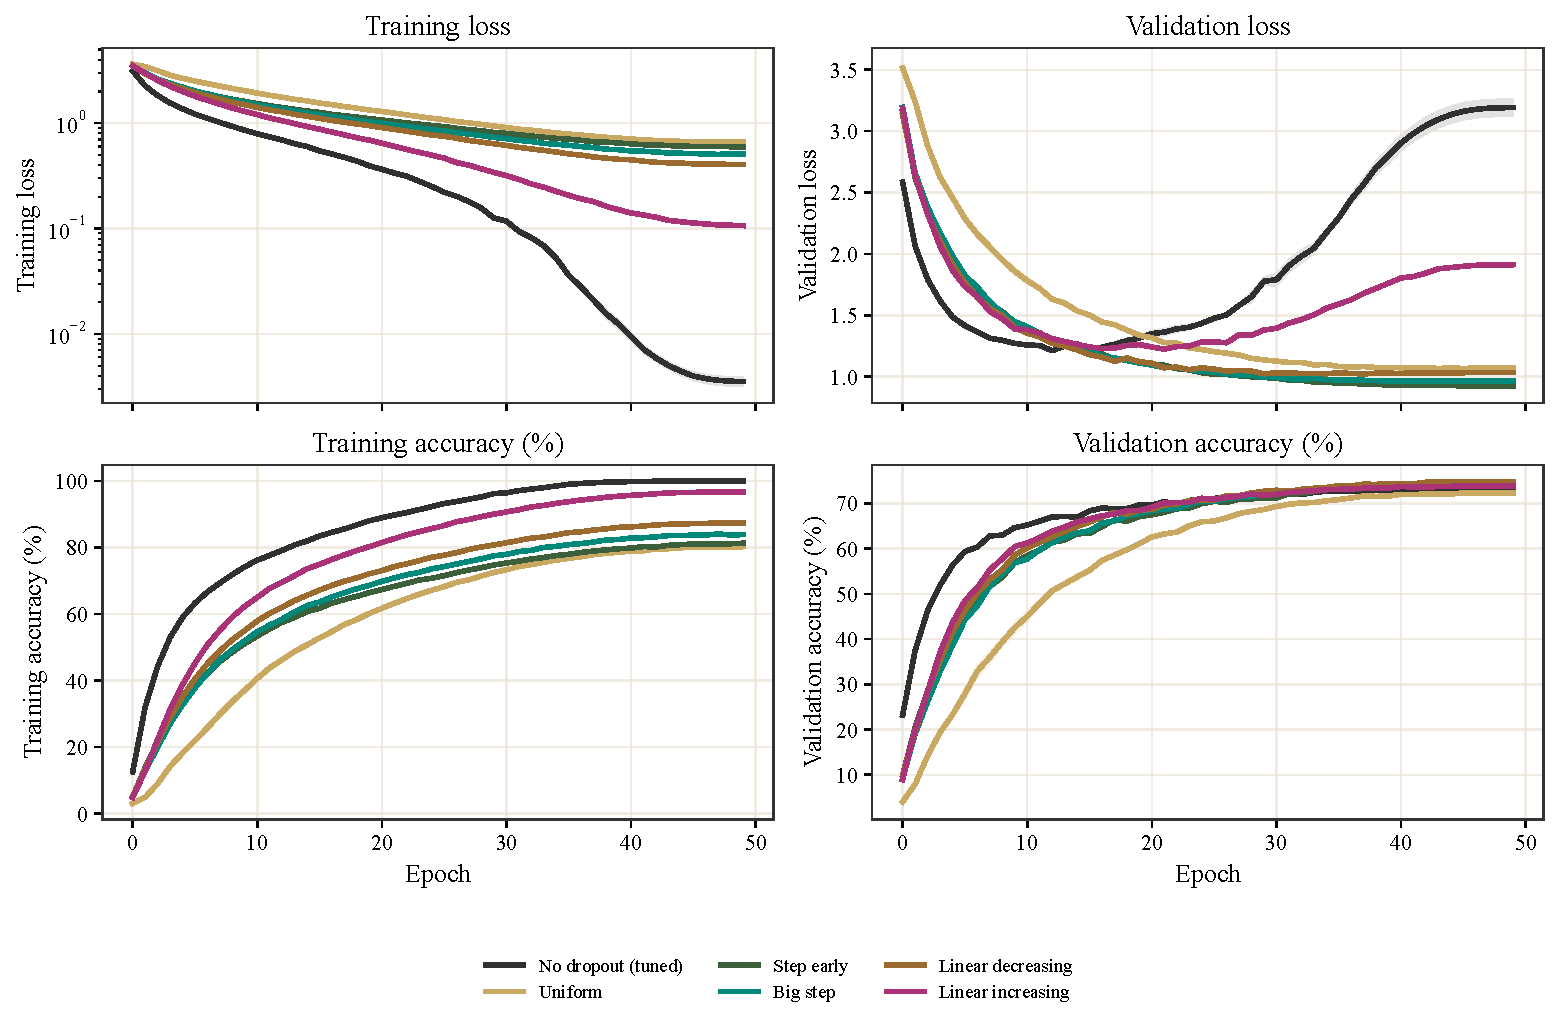
\includegraphics[width=0.92\textwidth]{figures/experiments/benchmarks/speech-commands-mlp.pdf}
\caption{Speech Commands / MLP / Zero weight decay. Original-cohort learning curves; bands show SEM across the recorded seeds for each profile. Sample counts and tuned probabilities are given below.}
\label{fig:speech-commands-mlp}
\end{figure}
\begin{center}\small
\begin{tabular}{@{}lrrrrrr@{}}
\toprule
Profile & $n$ & $\bar p$ & Learning rate & Test CE & Test acc. (\%) & Final test CE \\
\midrule
No dropout (tuned) & 5 & 0.00 & 1e-03 & \(1.203\pm0.011\) & \(67.16\pm0.35\) & -- \\
Uniform & 5 & 0.10 & 1e-03 & \(1.073\pm0.006\) & \(72.23\pm0.12\) & -- \\
Step early & 5 & 0.05 & 1e-03 & \(0.937\pm0.003\) & \(74.06\pm0.13\) & -- \\
Big step & 5 & 0.05 & 1e-03 & \(0.950\pm0.004\) & \(74.07\pm0.11\) & -- \\
Linear decreasing & 5 & 0.05 & 1e-03 & \(1.002\pm0.005\) & \(73.87\pm0.45\) & -- \\
Linear increasing & 5 & 0.05 & 1e-03 & \(1.202\pm0.009\) & \(69.40\pm0.54\) & -- \\
\bottomrule\end{tabular}\end{center}
\emph{Test endpoints.} Test CE and accuracy use the minimum-validation-loss checkpoint. Dashes indicate that final-epoch test CE was not recorded in this original cohort; the final losses in the learning curves are validation losses.
For the validation-selected nonuniform profile, the paired test-CE difference (profile minus uniform) is \(-0.136\pm0.007\) (SEM).
\clearpage
\subsection{Speech Commands / Transformer / Zero weight decay}
Depth 12, width 256; 20,020/5,005/10,010 training/validation/test examples; 50 epochs, batch size 128, weight decay \(0\). The recorded split is held fixed across profiles.
\begin{figure}[ht]
\centering
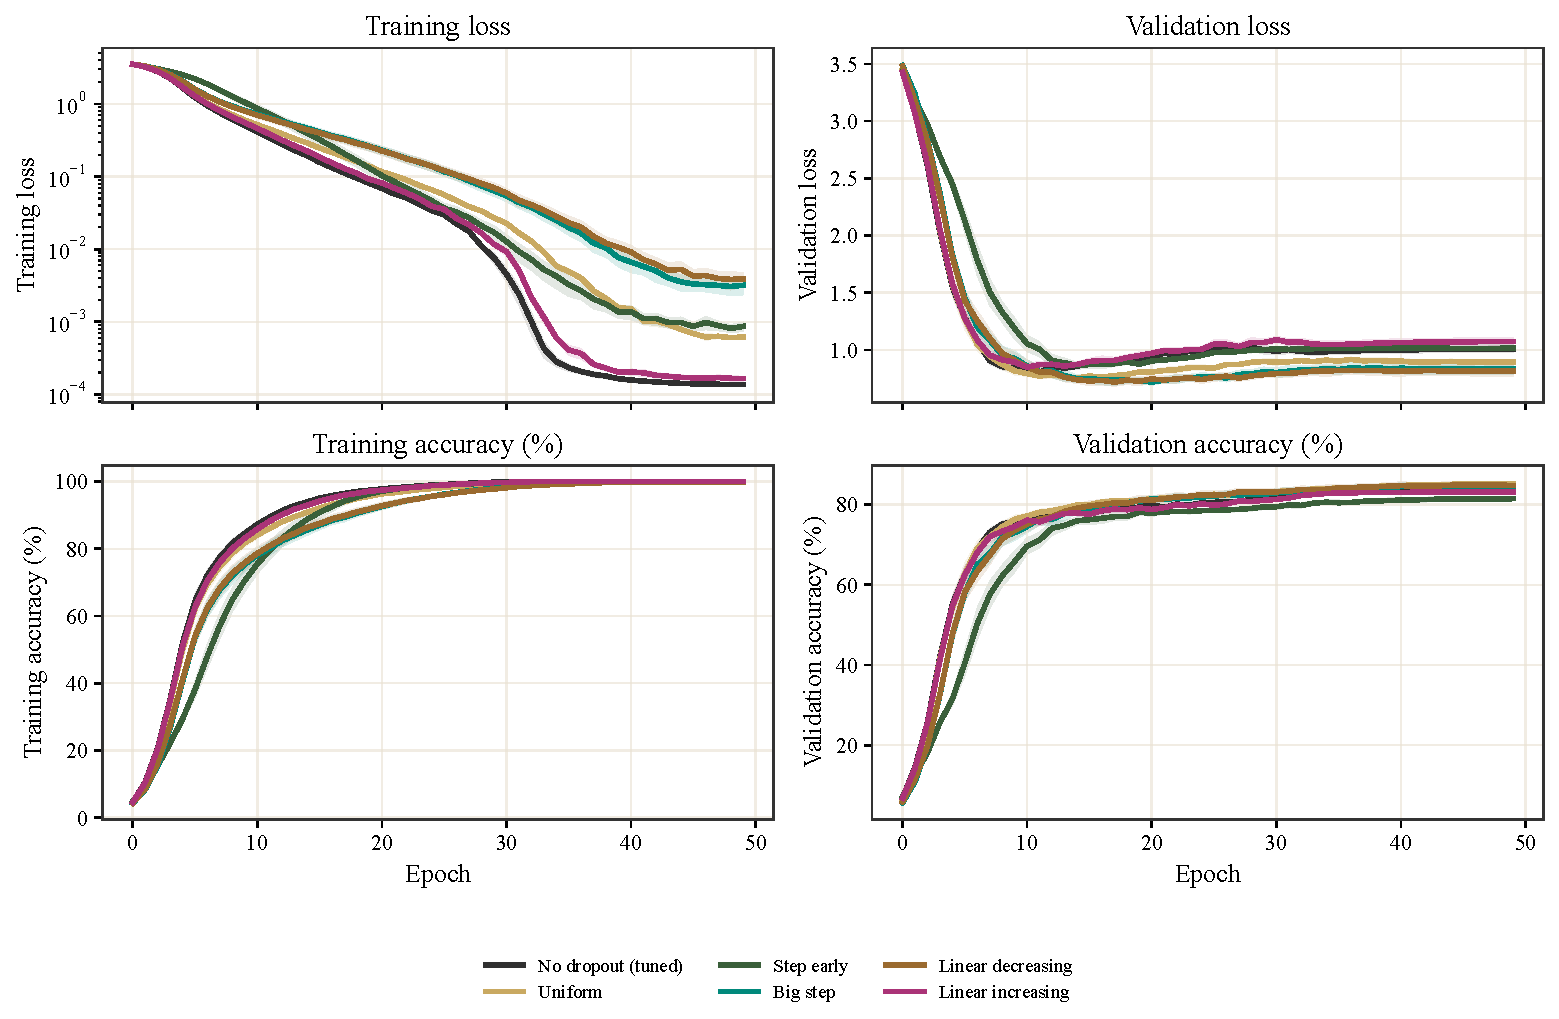
\includegraphics[width=0.92\textwidth]{figures/experiments/benchmarks/speech-commands-transformer.pdf}
\caption{Speech Commands / Transformer / Zero weight decay. Original-cohort learning curves; bands show SEM across the recorded seeds for each profile. Sample counts and tuned probabilities are given below.}
\label{fig:speech-commands-transformer}
\end{figure}
\begin{center}\small
\begin{tabular}{@{}lrrrrrr@{}}
\toprule
Profile & $n$ & $\bar p$ & Learning rate & Test CE & Test acc. (\%) & Final test CE \\
\midrule
No dropout (tuned) & 5 & 0.00 & 3e-04 & \(0.807\pm0.018\) & \(77.65\pm0.65\) & -- \\
Uniform & 5 & 0.15 & 3e-04 & \(0.743\pm0.017\) & \(79.54\pm0.61\) & -- \\
Step early & 5 & 0.05 & 1e-04 & \(0.852\pm0.027\) & \(77.85\pm0.64\) & -- \\
Big step & 5 & 0.15 & 3e-04 & \(0.707\pm0.036\) & \(81.07\pm0.89\) & -- \\
Linear decreasing & 5 & 0.20 & 3e-04 & \(0.711\pm0.033\) & \(81.27\pm1.05\) & -- \\
Linear increasing & 5 & 0.10 & 3e-04 & \(0.832\pm0.022\) & \(77.67\pm0.67\) & -- \\
\bottomrule\end{tabular}\end{center}
\emph{Test endpoints.} Test CE and accuracy use the minimum-validation-loss checkpoint. Dashes indicate that final-epoch test CE was not recorded in this original cohort; the final losses in the learning curves are validation losses.
For the validation-selected nonuniform profile, the paired test-CE difference (profile minus uniform) is \(-0.036\pm0.037\) (SEM).
\clearpage
\subsection{Tiny ImageNet / MLP / 80,000 train}
Depth 12, width 256; 80,000/10,000/10,000 training/validation/test examples; 75 epochs, batch size 128, weight decay \(0\). The recorded split is held fixed across profiles.
\begin{figure}[ht]
\centering
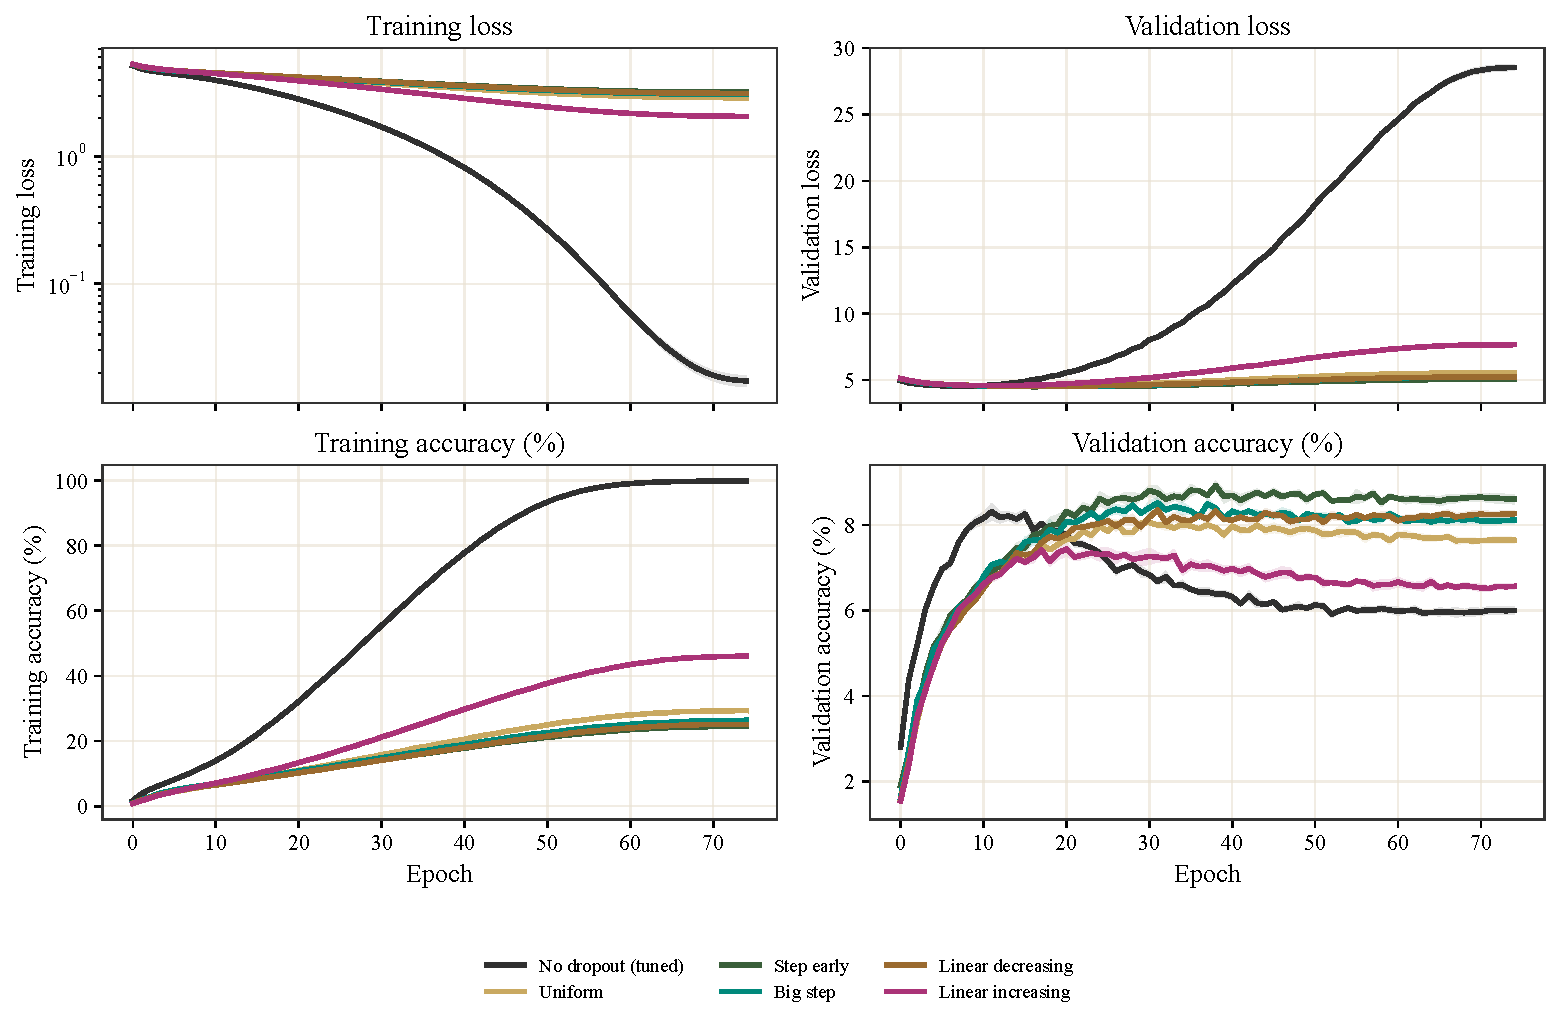
\includegraphics[width=0.92\textwidth]{figures/experiments/benchmarks/tiny-imagenet-mlp-80k.pdf}
\caption{Tiny ImageNet / MLP / 80,000 train. Original-cohort learning curves; bands show SEM across the recorded seeds for each profile. Sample counts and tuned probabilities are given below.}
\label{fig:tiny-imagenet-mlp-80k}
\end{figure}
\begin{center}\small
\begin{tabular}{@{}lrrrrrr@{}}
\toprule
Profile & $n$ & $\bar p$ & Learning rate & Test CE & Test acc. (\%) & Final test CE \\
\midrule
No dropout (tuned) & 5 & 0.00 & 3e-04 & \(4.561\pm0.004\) & \(7.64\pm0.15\) & \(28.876\pm0.230\) \\
Uniform & 5 & 0.05 & 3e-04 & \(4.575\pm0.002\) & \(7.09\pm0.14\) & \(5.627\pm0.004\) \\
Step early & 5 & 0.05 & 3e-04 & \(4.518\pm0.004\) & \(7.95\pm0.10\) & \(5.130\pm0.009\) \\
Big step & 5 & 0.05 & 3e-04 & \(4.541\pm0.003\) & \(7.53\pm0.12\) & \(5.321\pm0.007\) \\
Linear decreasing & 5 & 0.05 & 3e-04 & \(4.563\pm0.003\) & \(7.19\pm0.15\) & \(5.286\pm0.013\) \\
Linear increasing & 5 & 0.05 & 3e-04 & \(4.608\pm0.005\) & \(6.75\pm0.12\) & \(7.764\pm0.023\) \\
\bottomrule\end{tabular}\end{center}
For the validation-selected nonuniform profile, the paired test-CE difference (profile minus uniform) is \(-0.058\pm0.005\) (SEM).
\clearpage
\subsection{Tiny ImageNet / Transformer / 80,000 train}
Depth 12, width 256; 80,000/10,000/10,000 training/validation/test examples; 75 epochs, batch size 128, weight decay \(0\). The recorded split is held fixed across profiles.
\begin{figure}[ht]
\centering
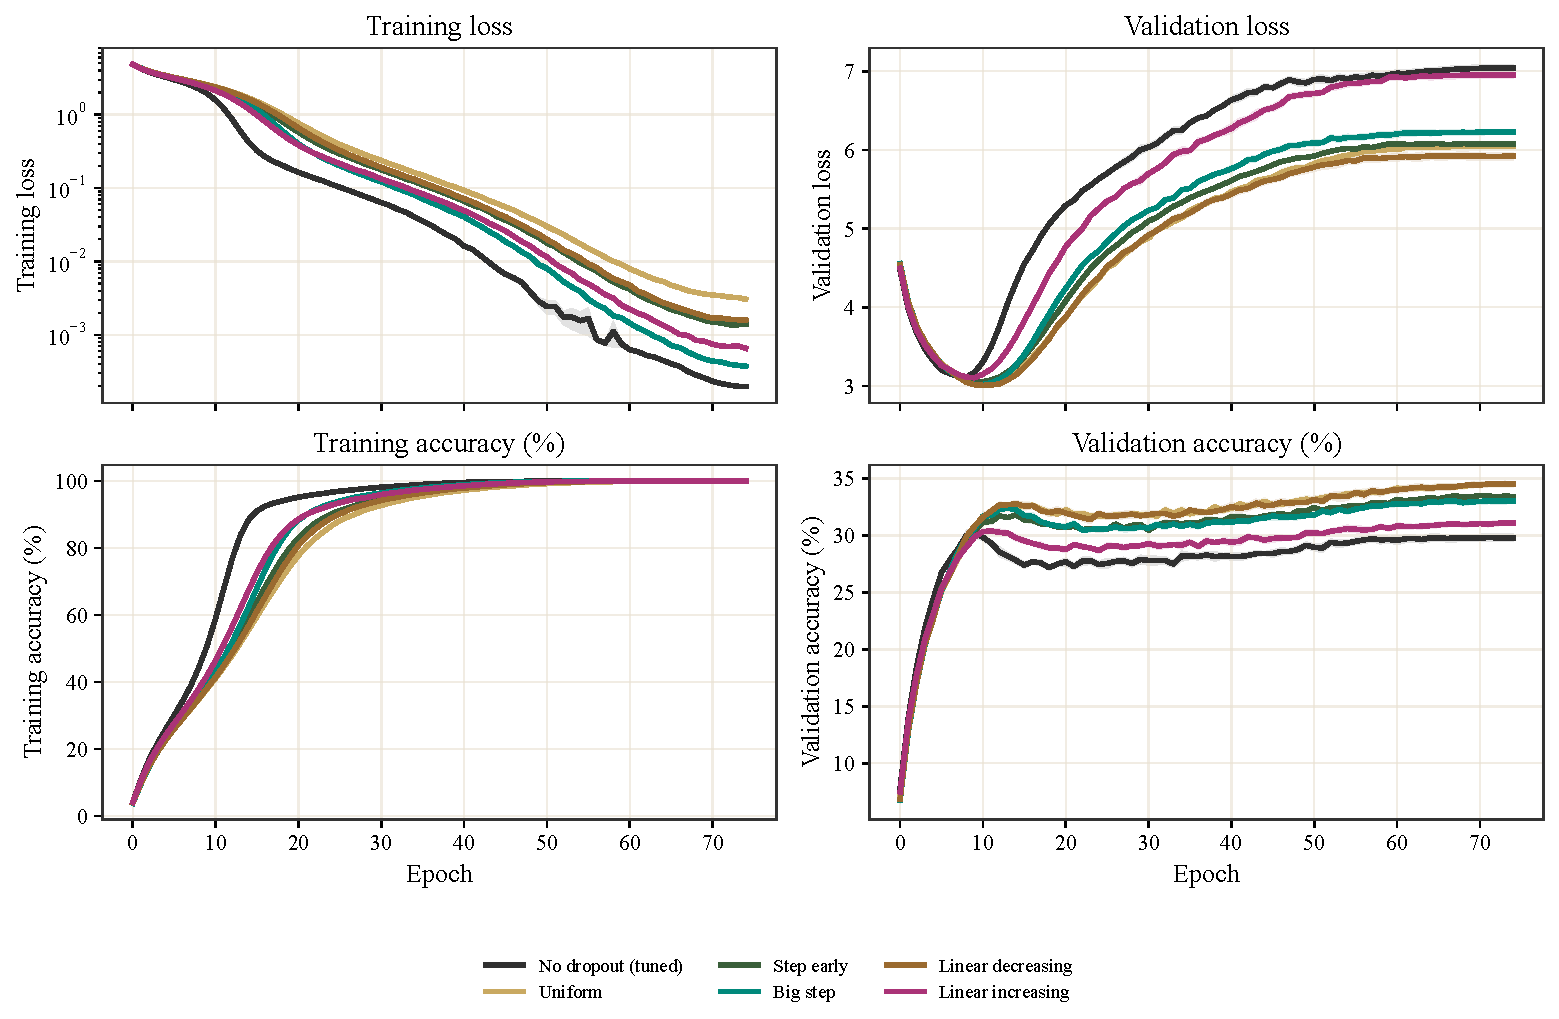
\includegraphics[width=0.92\textwidth]{figures/experiments/benchmarks/tiny-imagenet-transformer-80k.pdf}
\caption{Tiny ImageNet / Transformer / 80,000 train. Original-cohort learning curves; bands show SEM across the recorded seeds for each profile. Sample counts and tuned probabilities are given below.}
\label{fig:tiny-imagenet-transformer-80k}
\end{figure}
\begin{center}\small
\begin{tabular}{@{}lrrrrrr@{}}
\toprule
Profile & $n$ & $\bar p$ & Learning rate & Test CE & Test acc. (\%) & Final test CE \\
\midrule
No dropout (tuned) & 5 & 0.00 & 3e-04 & \(3.125\pm0.025\) & \(29.57\pm0.44\) & \(7.126\pm0.068\) \\
Uniform & 5 & 0.20 & 3e-04 & \(3.035\pm0.014\) & \(31.49\pm0.17\) & \(6.104\pm0.043\) \\
Step early & 5 & 0.15 & 3e-04 & \(3.053\pm0.015\) & \(31.22\pm0.21\) & \(6.164\pm0.025\) \\
Big step & 5 & 0.10 & 3e-04 & \(3.026\pm0.013\) & \(31.35\pm0.38\) & \(6.296\pm0.034\) \\
Linear decreasing & 5 & 0.15 & 3e-04 & \(3.004\pm0.016\) & \(31.78\pm0.23\) & \(6.002\pm0.042\) \\
Linear increasing & 5 & 0.20 & 3e-04 & \(3.118\pm0.017\) & \(29.72\pm0.26\) & \(7.026\pm0.052\) \\
\bottomrule\end{tabular}\end{center}
For the validation-selected nonuniform profile, the paired test-CE difference (profile minus uniform) is \(-0.031\pm0.015\) (SEM).
\clearpage
\subsection{FI-2010 / Transformer / Linear follow-up}
Depth 12, width 256; 40,000/10,000/20,000 training/validation/test examples; 50 epochs, batch size 128, weight decay \(1e-07\). The recorded split is held fixed across profiles.
\begin{figure}[ht]
\centering
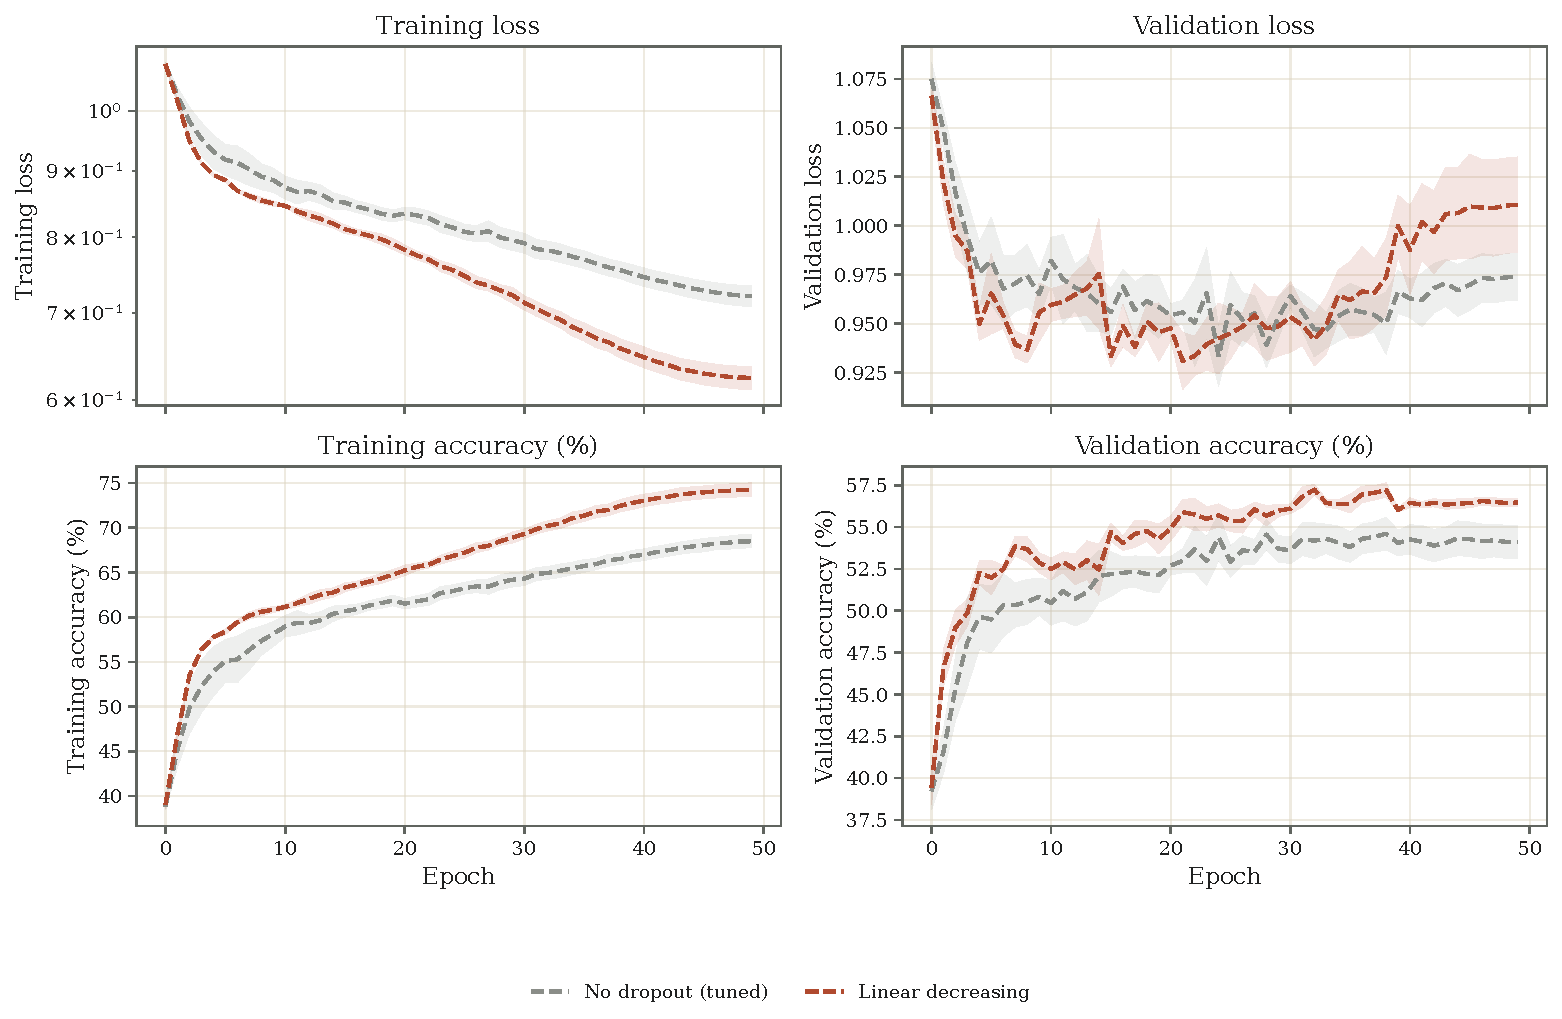
\includegraphics[width=0.92\textwidth]{figures/experiments/benchmarks/fi2010-transformer-linear.pdf}
\caption{FI-2010 / Transformer / Linear follow-up. Original-cohort learning curves; bands show SEM across the recorded seeds for each profile. Sample counts and tuned probabilities are given below.}
\label{fig:fi2010-transformer-linear}
\end{figure}
\begin{center}\small
\begin{tabular}{@{}lrrrrrr@{}}
\toprule
Profile & $n$ & $\bar p$ & Learning rate & Test CE & Test acc. (\%) & Final test CE \\
\midrule
No dropout (tuned) & 5 & 0.00 & 1e-03 & \(0.955\pm0.010\) & \(55.38\pm0.39\) & -- \\
Linear decreasing & 5 & 0.10 & 1e-03 & \(0.930\pm0.006\) & \(57.72\pm0.83\) & -- \\
\bottomrule\end{tabular}\end{center}
\clearpage
\subsection{Jannis / Transformer / Linear follow-up}
Depth 12, width 256; 3,840/960/1,920 training/validation/test examples; 50 epochs, batch size 128, weight decay \(1e-07\). The recorded split is held fixed across profiles.
\begin{figure}[ht]
\centering
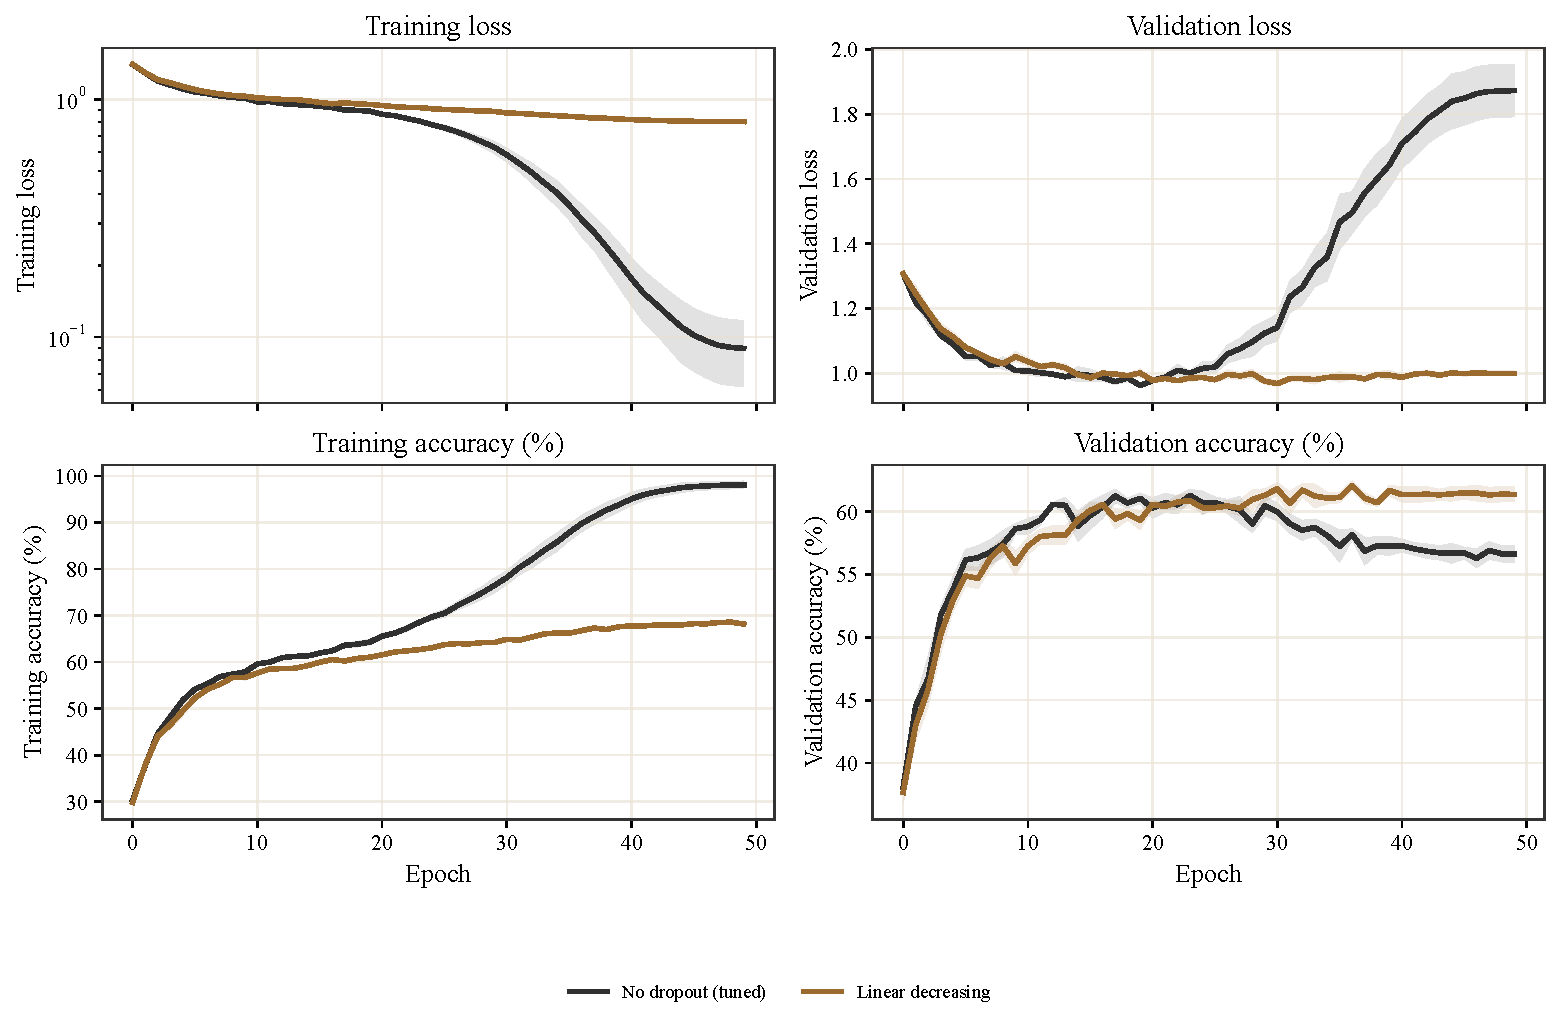
\includegraphics[width=0.92\textwidth]{figures/experiments/benchmarks/jannis-transformer-linear.pdf}
\caption{Jannis / Transformer / Linear follow-up. Original-cohort learning curves; bands show SEM across the recorded seeds for each profile. Sample counts and tuned probabilities are given below.}
\label{fig:jannis-transformer-linear}
\end{figure}
\begin{center}\small
\begin{tabular}{@{}lrrrrrr@{}}
\toprule
Profile & $n$ & $\bar p$ & Learning rate & Test CE & Test acc. (\%) & Final test CE \\
\midrule
No dropout (tuned) & 5 & 0.00 & 1e-04 & \(0.986\pm0.002\) & \(59.07\pm0.47\) & -- \\
Linear decreasing & 5 & 0.10 & 1e-04 & \(0.992\pm0.005\) & \(60.27\pm0.43\) & -- \\
\bottomrule\end{tabular}\end{center}
\clearpage
\subsection{Jannis / Transformer / 100 epochs}
Depth 12, width 256; 3,840/960/1,920 training/validation/test examples; 100 epochs, batch size 128, weight decay \(1e-07\). The recorded split is held fixed across profiles.
\begin{figure}[ht]
\centering
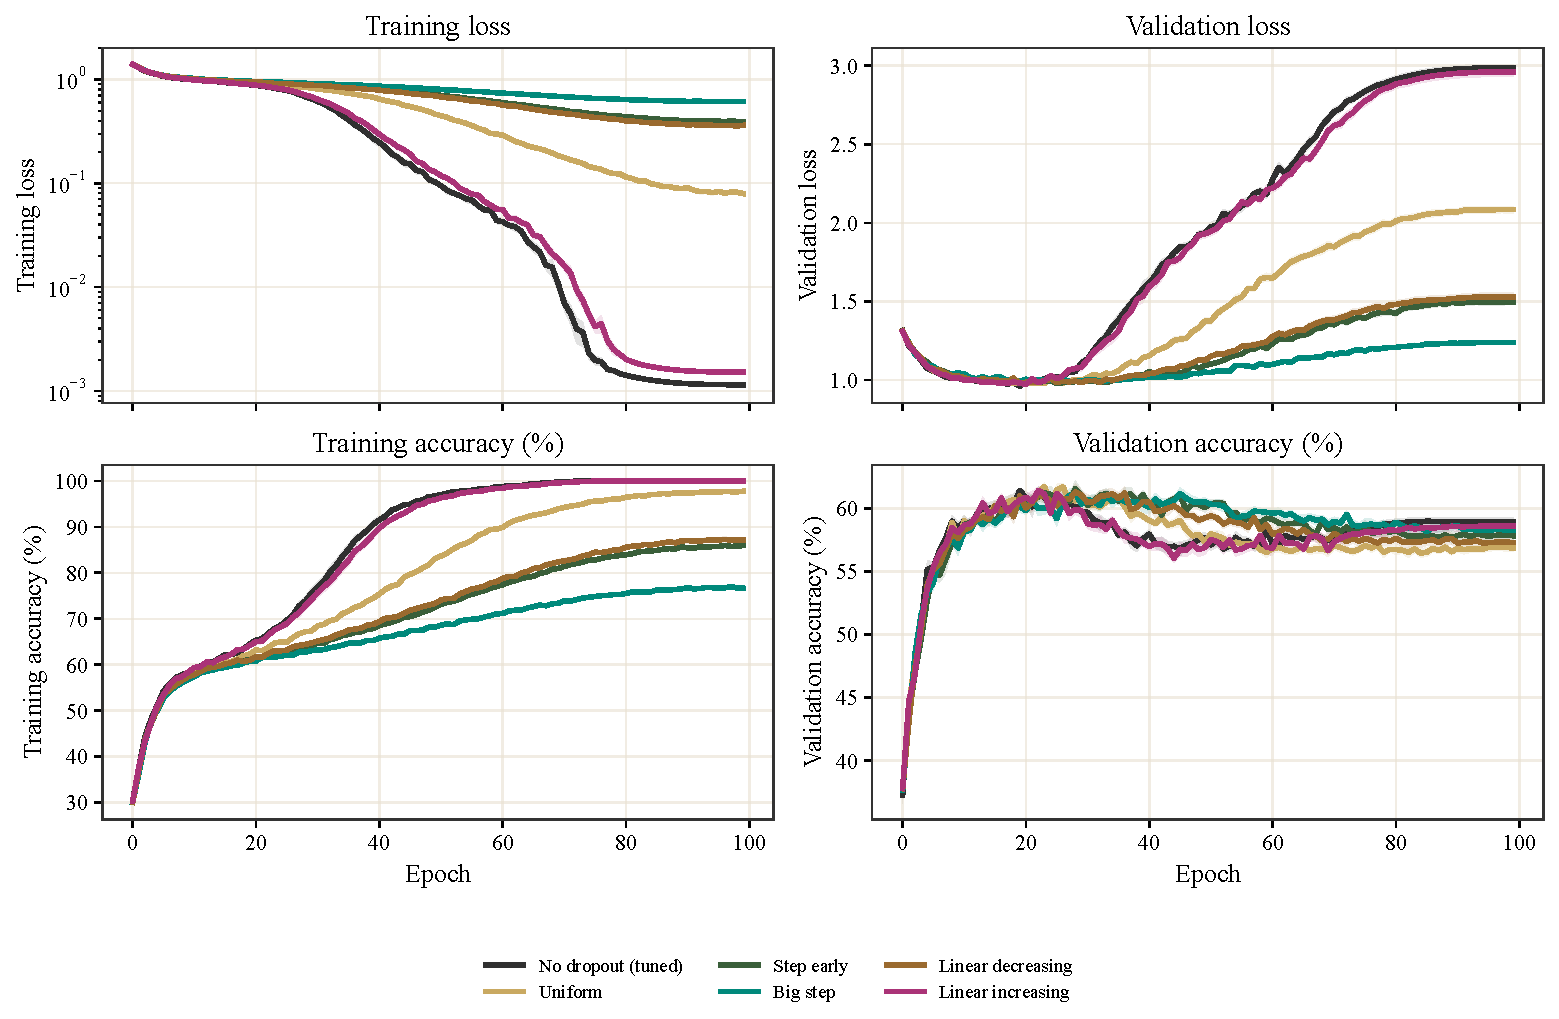
\includegraphics[width=0.92\textwidth]{figures/experiments/benchmarks/jannis-transformer-100-epochs.pdf}
\caption{Jannis / Transformer / 100 epochs. Original-cohort learning curves; bands show SEM across the recorded seeds for each profile. Sample counts and tuned probabilities are given below.}
\label{fig:jannis-transformer-100-epochs}
\end{figure}
\begin{center}\small
\begin{tabular}{@{}lrrrrrr@{}}
\toprule
Profile & $n$ & $\bar p$ & Learning rate & Test CE & Test acc. (\%) & Final test CE \\
\midrule
No dropout (tuned) & 10 & 0.00 & 1e-04 & \(0.985\pm0.003\) & \(59.54\pm0.16\) & -- \\
Uniform & 10 & 0.10 & 1e-04 & \(0.988\pm0.002\) & \(59.46\pm0.23\) & -- \\
Step early & 10 & 0.10 & 1e-04 & \(0.990\pm0.004\) & \(59.85\pm0.21\) & -- \\
Big step & 10 & 0.10 & 1e-04 & \(0.999\pm0.003\) & \(59.36\pm0.29\) & -- \\
Linear decreasing & 10 & 0.10 & 1e-04 & \(0.988\pm0.003\) & \(59.75\pm0.13\) & -- \\
Linear increasing & 10 & 0.10 & 1e-04 & \(0.992\pm0.003\) & \(59.40\pm0.25\) & -- \\
\bottomrule\end{tabular}\end{center}
For the validation-selected nonuniform profile, the paired test-CE difference (profile minus uniform) is \(0.004\pm0.003\) (SEM).
\clearpage
\subsection{Tiny ImageNet / MLP / Zero weight decay}
Depth 12, width 256; 20,000/5,000/10,000 training/validation/test examples; 75 epochs, batch size 128, weight decay \(0\). The recorded split is held fixed across profiles.
\begin{figure}[ht]
\centering
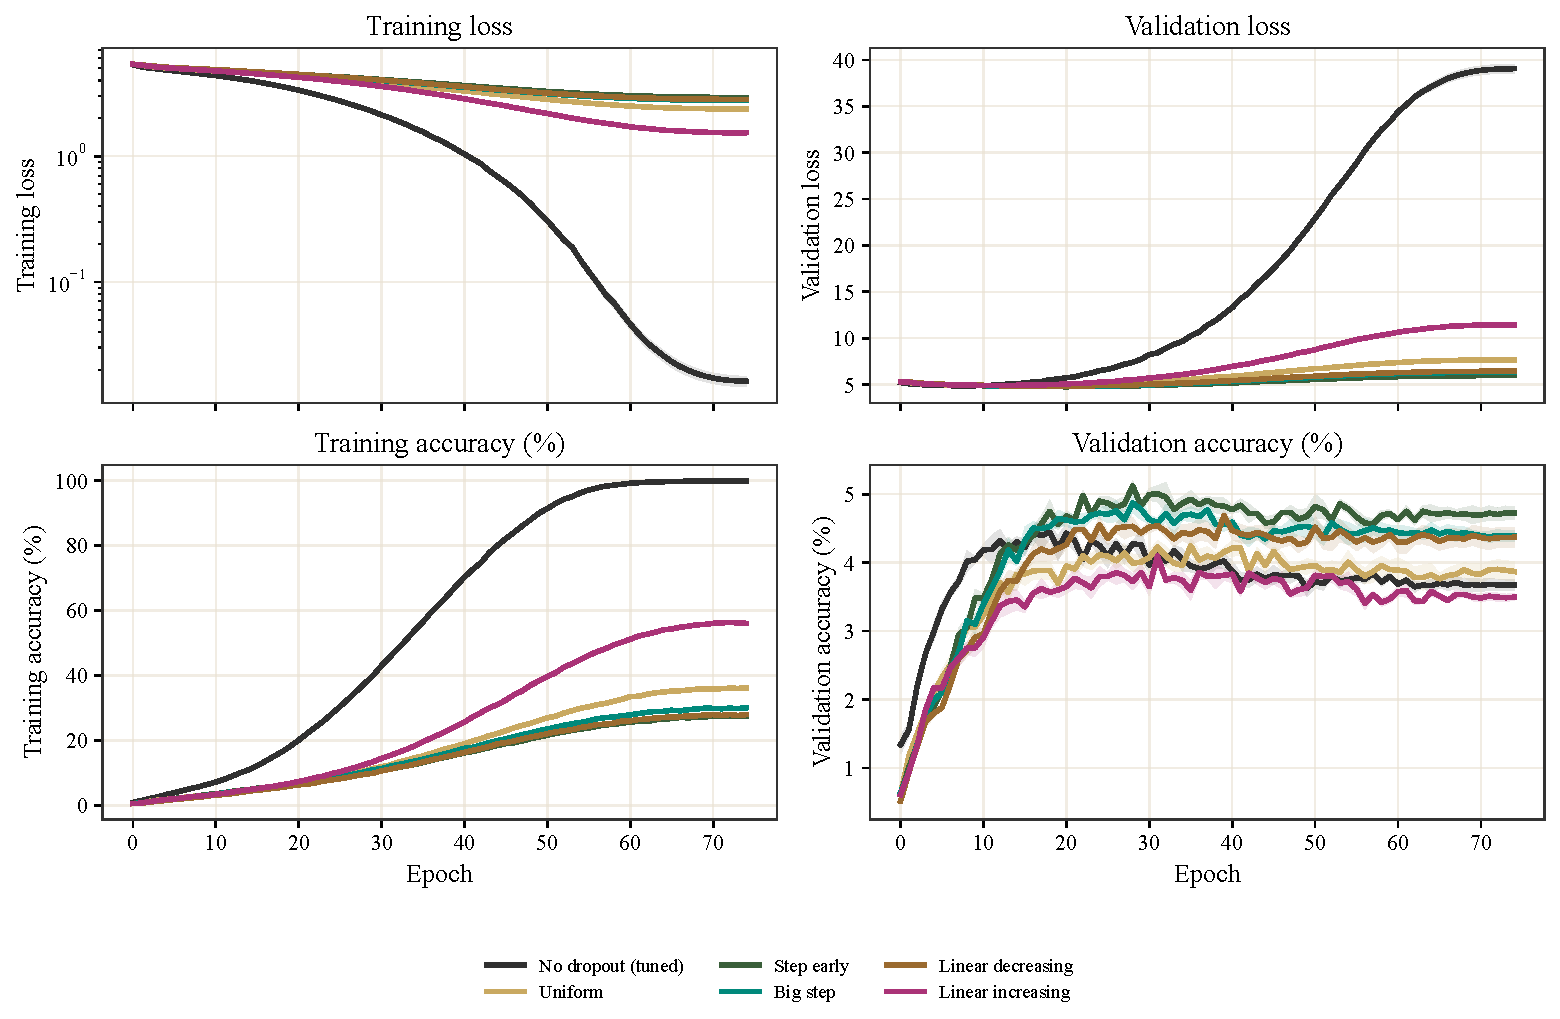
\includegraphics[width=0.92\textwidth]{figures/experiments/benchmarks/tiny-imagenet-mlp-20k.pdf}
\caption{Tiny ImageNet / MLP / Zero weight decay. Original-cohort learning curves; bands show SEM across the recorded seeds for each profile. Sample counts and tuned probabilities are given below.}
\label{fig:tiny-imagenet-mlp-20k}
\end{figure}
\begin{center}\small
\begin{tabular}{@{}lrrrrrr@{}}
\toprule
Profile & $n$ & $\bar p$ & Learning rate & Test CE & Test acc. (\%) & Final test CE \\
\midrule
No dropout (tuned) & 5 & 0.00 & 1e-03 & \(4.856\pm0.005\) & \(3.88\pm0.05\) & -- \\
Uniform & 5 & 0.05 & 1e-03 & \(4.868\pm0.006\) & \(3.45\pm0.06\) & -- \\
Step early & 5 & 0.05 & 3e-04 & \(4.774\pm0.006\) & \(4.84\pm0.04\) & -- \\
Big step & 5 & 0.05 & 3e-04 & \(4.787\pm0.003\) & \(4.61\pm0.10\) & -- \\
Linear decreasing & 5 & 0.05 & 3e-04 & \(4.823\pm0.004\) & \(4.38\pm0.10\) & -- \\
Linear increasing & 5 & 0.05 & 1e-03 & \(4.898\pm0.007\) & \(3.36\pm0.09\) & -- \\
\bottomrule\end{tabular}\end{center}
For the validation-selected nonuniform profile, the paired test-CE difference (profile minus uniform) is \(-0.094\pm0.011\) (SEM).
\clearpage
\subsection{Tiny ImageNet / Transformer / Zero weight decay}
Depth 12, width 256; 20,000/5,000/10,000 training/validation/test examples; 75 epochs, batch size 128, weight decay \(0\). The recorded split is held fixed across profiles.
\begin{figure}[ht]
\centering
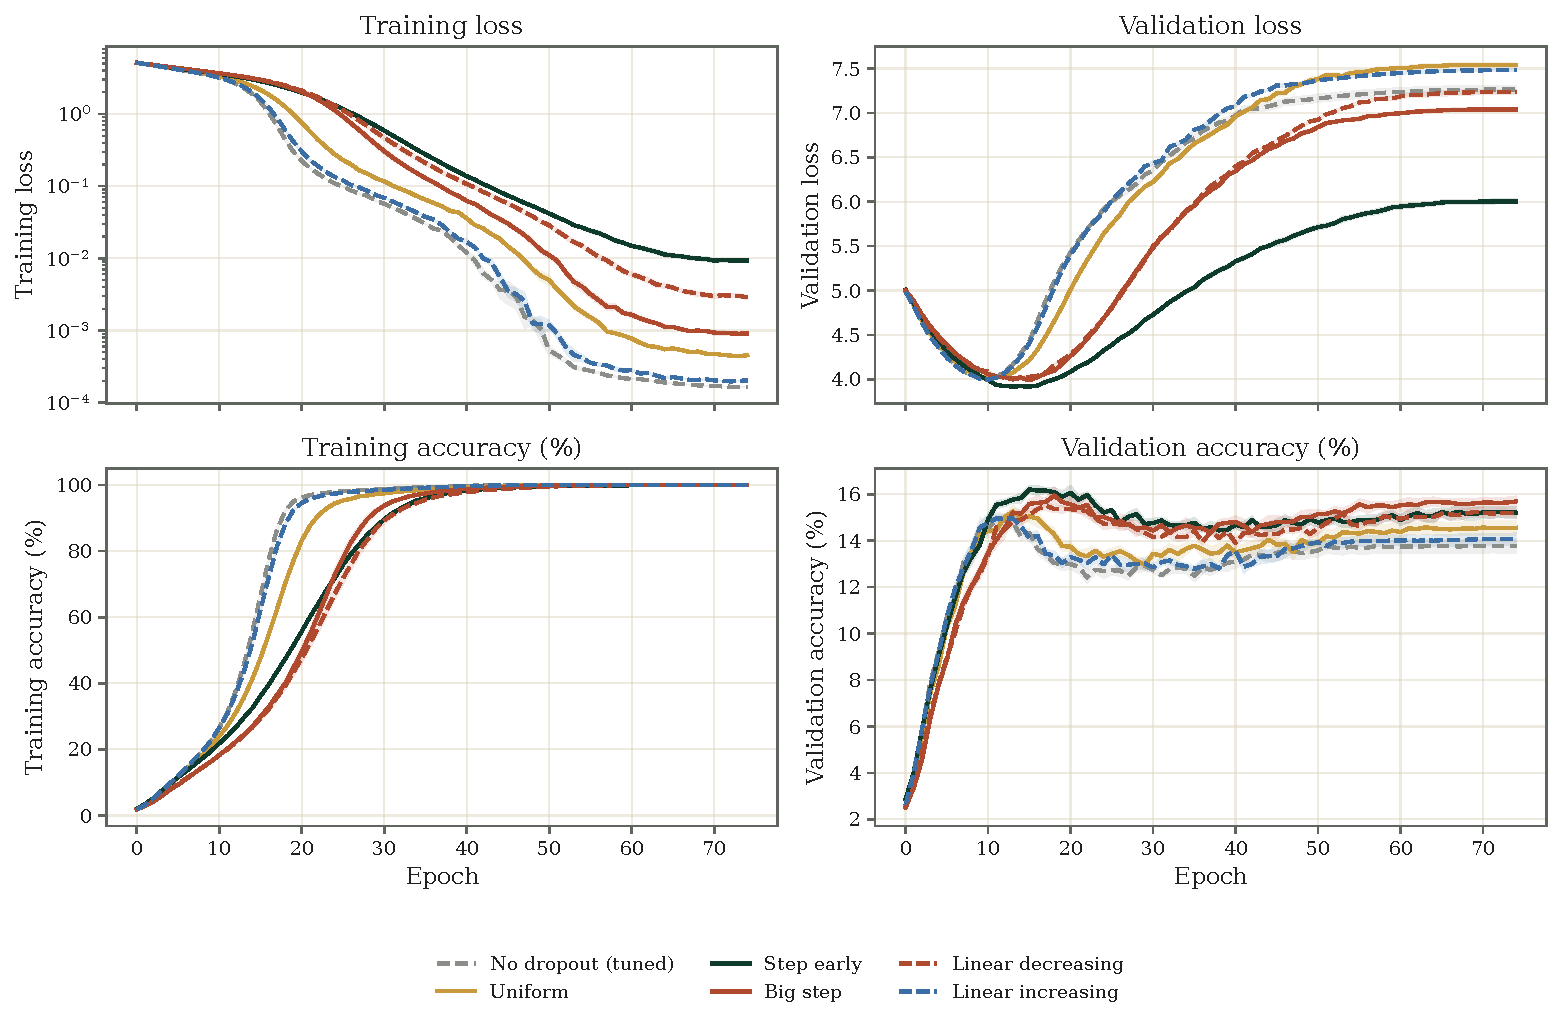
\includegraphics[width=0.92\textwidth]{figures/experiments/benchmarks/tiny-imagenet-transformer-20k.pdf}
\caption{Tiny ImageNet / Transformer / Zero weight decay. Original-cohort learning curves; bands show SEM across the recorded seeds for each profile. Sample counts and tuned probabilities are given below.}
\label{fig:tiny-imagenet-transformer-20k}
\end{figure}
\begin{center}\small
\begin{tabular}{@{}lrrrrrr@{}}
\toprule
Profile & $n$ & $\bar p$ & Learning rate & Test CE & Test acc. (\%) & Final test CE \\
\midrule
No dropout (tuned) & 5 & 0.00 & 3e-04 & \(3.981\pm0.012\) & \(14.92\pm0.21\) & -- \\
Uniform & 5 & 0.10 & 3e-04 & \(3.976\pm0.007\) & \(14.63\pm0.17\) & -- \\
Step early & 5 & 0.15 & 1e-04 & \(3.890\pm0.008\) & \(16.26\pm0.10\) & -- \\
Big step & 5 & 0.15 & 3e-04 & \(3.960\pm0.012\) & \(15.45\pm0.29\) & -- \\
Linear decreasing & 5 & 0.20 & 3e-04 & \(3.980\pm0.011\) & \(14.71\pm0.22\) & -- \\
Linear increasing & 5 & 0.05 & 3e-04 & \(3.981\pm0.017\) & \(14.73\pm0.30\) & -- \\
\bottomrule\end{tabular}\end{center}
For the validation-selected nonuniform profile, the paired test-CE difference (profile minus uniform) is \(-0.086\pm0.013\) (SEM).
\clearpage
\subsection{FI-2010 / MLP / Zero weight decay}
Depth 12, width 256; 40,000/10,000/20,000 training/validation/test examples; 50 epochs, batch size 128, weight decay \(0\). The recorded split is held fixed across profiles.
\begin{figure}[ht]
\centering
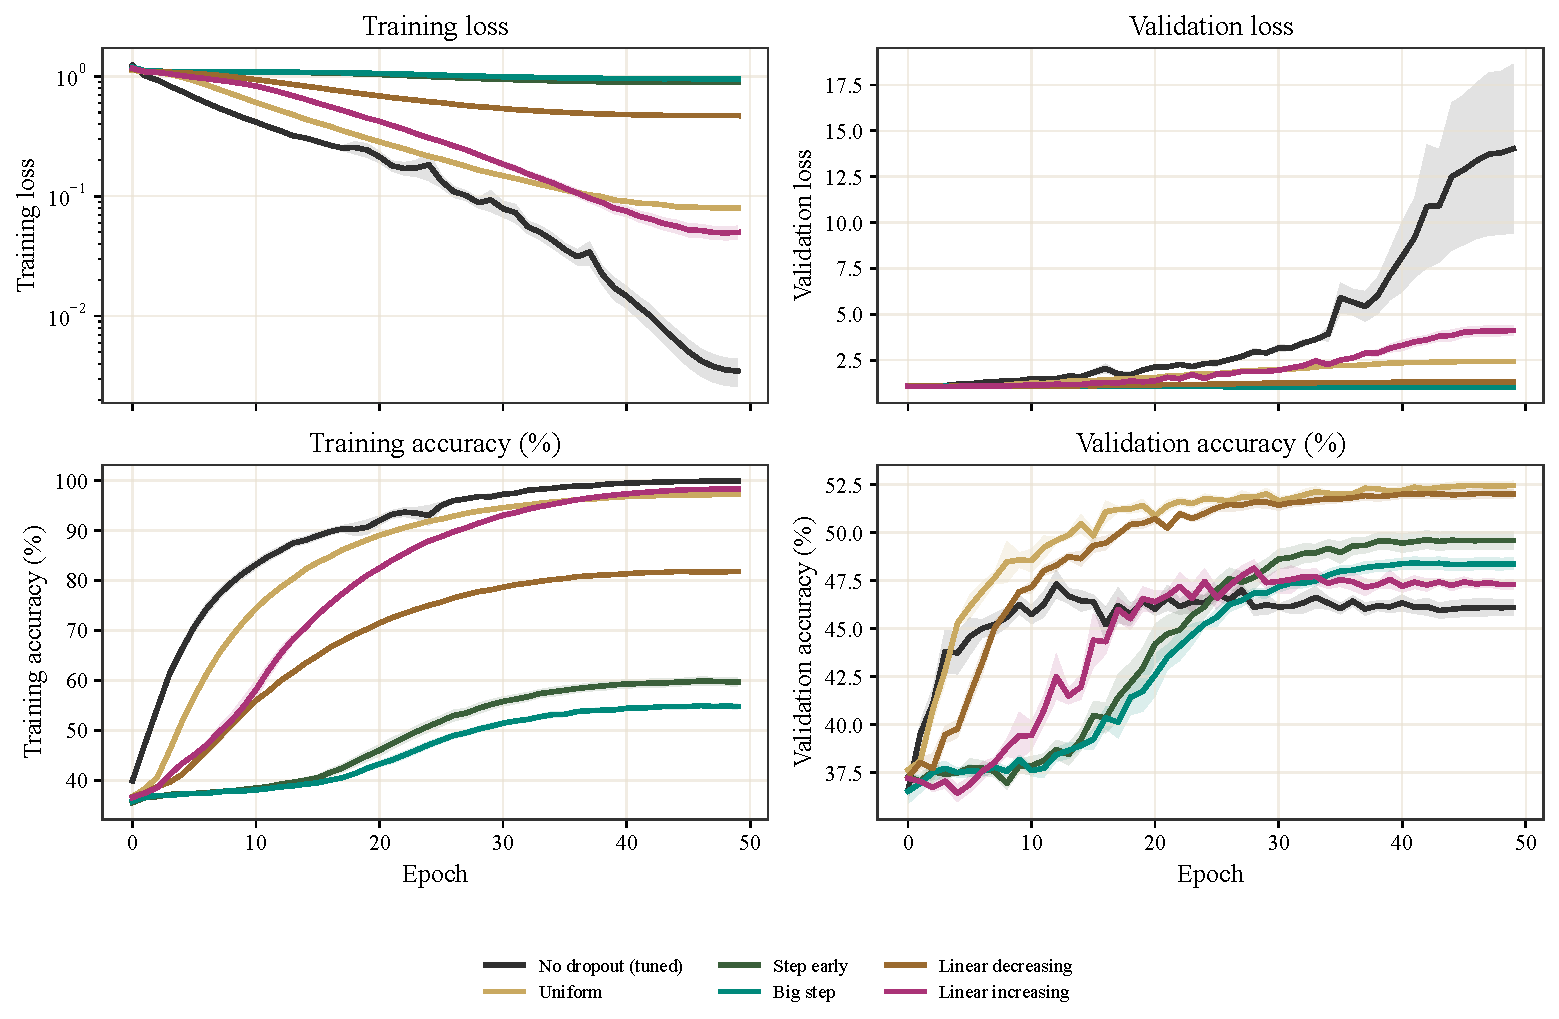
\includegraphics[width=0.92\textwidth]{figures/experiments/benchmarks/fi2010-mlp.pdf}
\caption{FI-2010 / MLP / Zero weight decay. Original-cohort learning curves; bands show SEM across the recorded seeds for each profile. Sample counts and tuned probabilities are given below.}
\label{fig:fi2010-mlp}
\end{figure}
\begin{center}\small
\begin{tabular}{@{}lrrrrrr@{}}
\toprule
Profile & $n$ & $\bar p$ & Learning rate & Test CE & Test acc. (\%) & Final test CE \\
\midrule
No dropout (tuned) & 5 & 0.00 & 3e-03 & \(1.118\pm0.017\) & \(42.19\pm2.20\) & -- \\
Uniform & 5 & 0.05 & 1e-04 & \(1.093\pm0.004\) & \(47.70\pm0.37\) & -- \\
Step early & 5 & 0.10 & 3e-05 & \(1.061\pm0.004\) & \(48.19\pm0.33\) & -- \\
Big step & 5 & 0.10 & 3e-05 & \(1.054\pm0.004\) & \(48.37\pm0.39\) & -- \\
Linear decreasing & 5 & 0.05 & 3e-05 & \(1.074\pm0.008\) & \(47.48\pm0.27\) & -- \\
Linear increasing & 5 & 0.15 & 1e-03 & \(1.115\pm0.011\) & \(37.62\pm0.39\) & -- \\
\bottomrule\end{tabular}\end{center}
For the validation-selected nonuniform profile, the paired test-CE difference (profile minus uniform) is \(-0.039\pm0.005\) (SEM).
\clearpage
\subsection{Jannis / MLP / Zero weight decay}
Depth 12, width 256; 3,840/960/1,920 training/validation/test examples; 100 epochs, batch size 128, weight decay \(0\). The recorded split is held fixed across profiles.
\begin{figure}[ht]
\centering
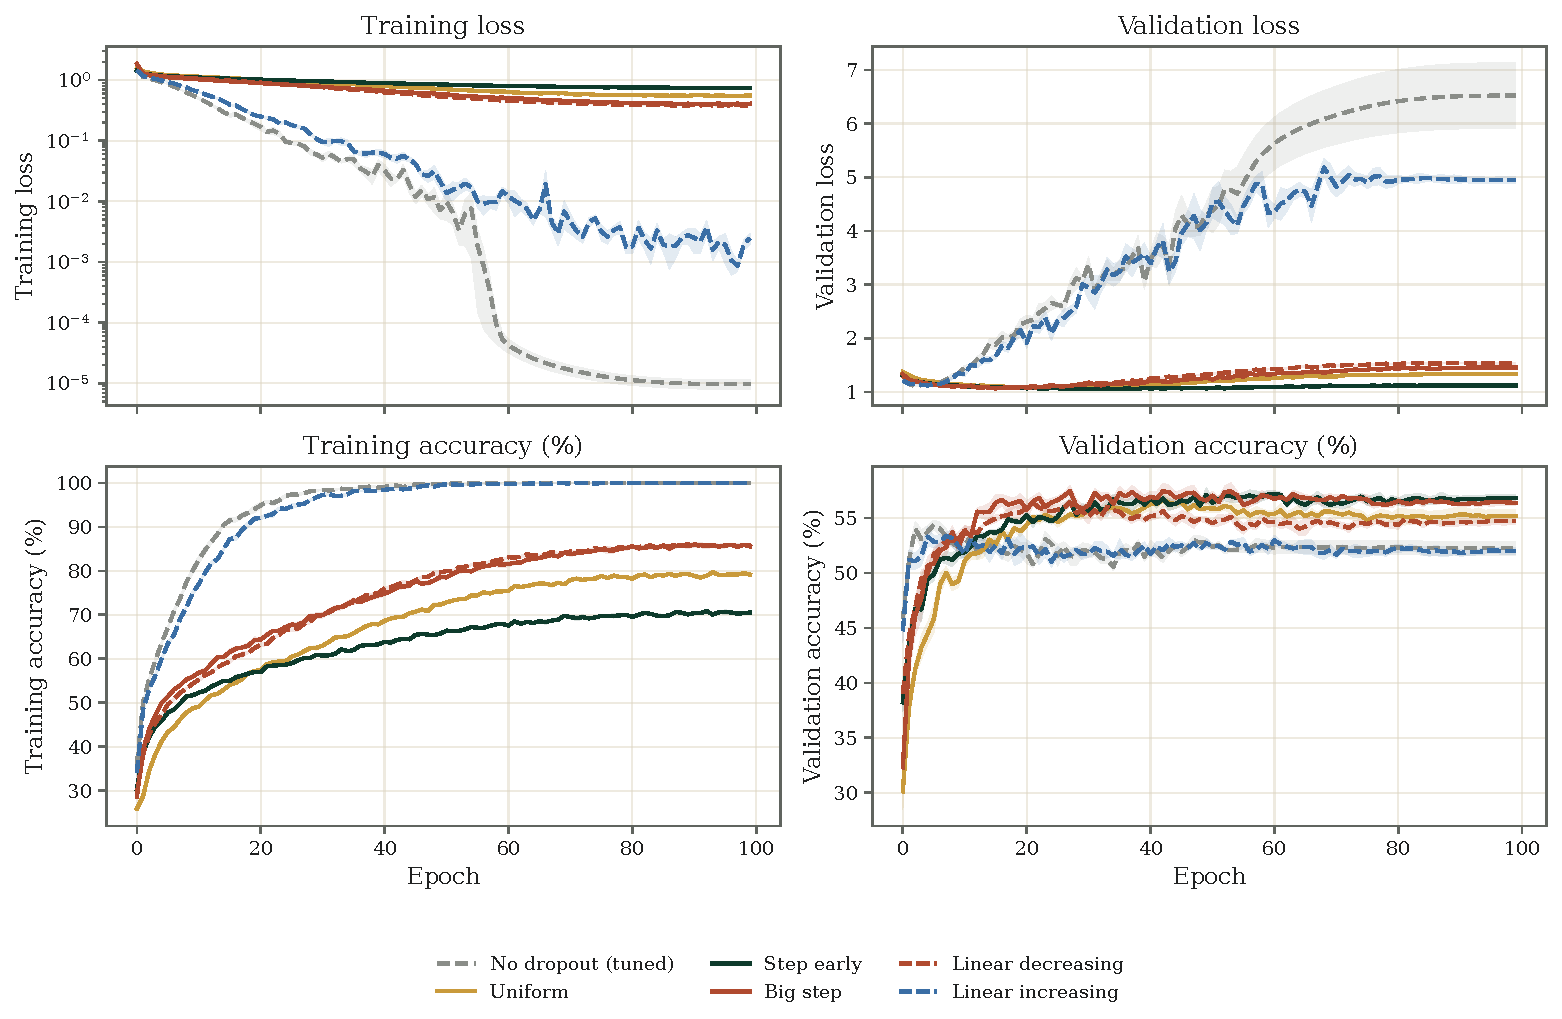
\includegraphics[width=0.92\textwidth]{figures/experiments/benchmarks/jannis-mlp.pdf}
\caption{Jannis / MLP / Zero weight decay. Original-cohort learning curves; bands show SEM across the recorded seeds for each profile. Sample counts and tuned probabilities are given below.}
\label{fig:jannis-mlp}
\end{figure}
\begin{center}\small
\begin{tabular}{@{}lrrrrrr@{}}
\toprule
Profile & $n$ & $\bar p$ & Learning rate & Test CE & Test acc. (\%) & Final test CE \\
\midrule
No dropout (tuned) & 5 & 0.00 & 3e-03 & \(1.123\pm0.006\) & \(51.56\pm0.38\) & -- \\
Uniform & 5 & 0.10 & 3e-04 & \(1.123\pm0.007\) & \(52.96\pm0.20\) & -- \\
Step early & 5 & 0.05 & 3e-04 & \(1.091\pm0.004\) & \(54.25\pm0.41\) & -- \\
Big step & 5 & 0.10 & 3e-03 & \(1.087\pm0.003\) & \(55.00\pm0.43\) & -- \\
Linear decreasing & 5 & 0.05 & 3e-04 & \(1.110\pm0.004\) & \(53.18\pm0.52\) & -- \\
Linear increasing & 5 & 0.05 & 3e-03 & \(1.140\pm0.008\) & \(51.77\pm0.71\) & -- \\
\bottomrule\end{tabular}\end{center}
For the validation-selected nonuniform profile, the paired test-CE difference (profile minus uniform) is \(-0.033\pm0.010\) (SEM).
\clearpage
\subsection{Jannis / Transformer / Zero weight decay}
Depth 12, width 256; 3,840/960/1,920 training/validation/test examples; 100 epochs, batch size 128, weight decay \(0\). The recorded split is held fixed across profiles.
\begin{figure}[ht]
\centering
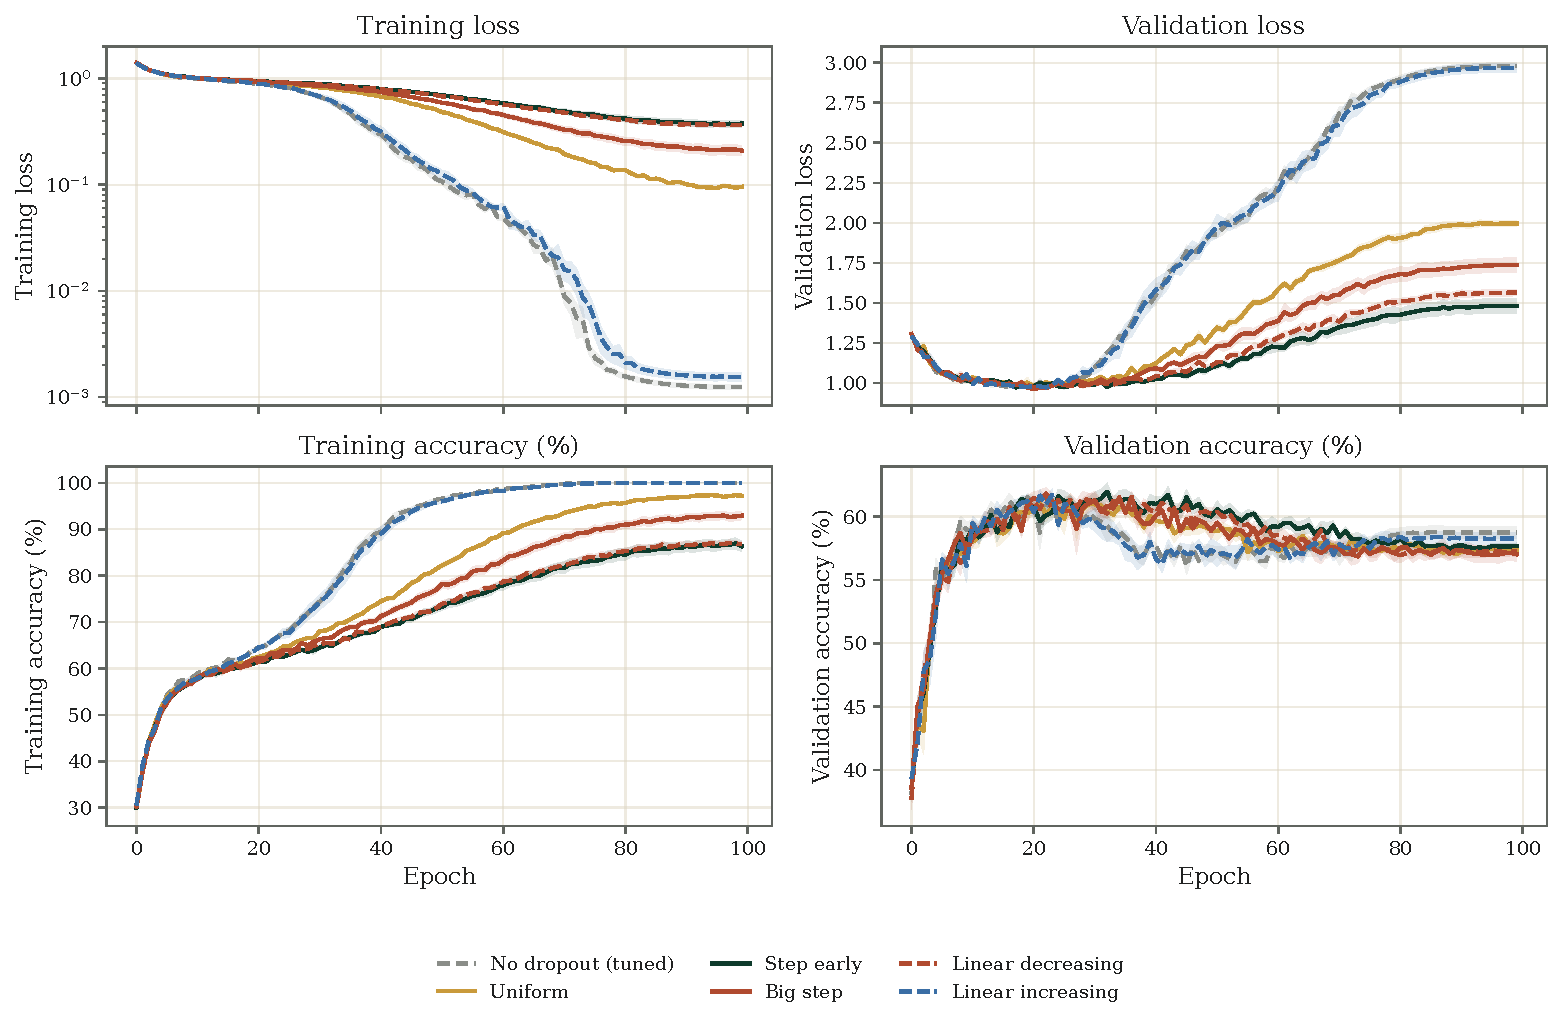
\includegraphics[width=0.92\textwidth]{figures/experiments/benchmarks/jannis-transformer.pdf}
\caption{Jannis / Transformer / Zero weight decay. Original-cohort learning curves; bands show SEM across the recorded seeds for each profile. Sample counts and tuned probabilities are given below.}
\label{fig:jannis-transformer}
\end{figure}
\begin{center}\small
\begin{tabular}{@{}lrrrrrr@{}}
\toprule
Profile & $n$ & $\bar p$ & Learning rate & Test CE & Test acc. (\%) & Final test CE \\
\midrule
No dropout (tuned) & 5 & 0.00 & 1e-04 & \(0.985\pm0.002\) & \(59.50\pm0.10\) & -- \\
Uniform & 5 & 0.10 & 1e-04 & \(0.993\pm0.004\) & \(58.98\pm0.19\) & -- \\
Step early & 5 & 0.05 & 1e-04 & \(0.988\pm0.001\) & \(59.22\pm0.21\) & -- \\
Big step & 5 & 0.05 & 1e-04 & \(0.992\pm0.003\) & \(59.24\pm0.57\) & -- \\
Linear decreasing & 5 & 0.10 & 1e-04 & \(0.994\pm0.003\) & \(58.90\pm0.32\) & -- \\
Linear increasing & 5 & 0.10 & 1e-04 & \(0.988\pm0.003\) & \(60.28\pm0.26\) & -- \\
\bottomrule\end{tabular}\end{center}
For the validation-selected nonuniform profile, the paired test-CE difference (profile minus uniform) is \(-0.002\pm0.005\) (SEM).
\clearpage
\subsection{Standalone FI-2010 vanilla MLPs}
These plain feedforward ReLU MLPs flatten a $128\times40$ input window. The study uses day 6 for training, day 7 for validation, and days 8--10 for test. Each architecture is trained for 100 epochs with five paired confirmation seeds (100--104), zero weight decay, and mean dropout $0.10$ for nonzero profiles. Weights have variance $1.98/\mathrm{fan\_in}$ and biases variance $0.02$. The learning rate is chosen using uniform-dropout validation runs and then held fixed across profiles, including no dropout. These are separate from the depth-12 width-256 benchmark cohorts.
Test loss, accuracy, and macro-F1 are evaluated once, at the minimum-validation-loss checkpoint. The saved results contain profile means and SEMs, but no validation objectives, per-seed test metrics, or per-epoch test histories. Final-epoch and minimum-over-training test losses are therefore unavailable. The standalone rows in Table~\ref{tab:benchmark_results} retain the retrospective choice of the nonuniform profile with the lowest observed mean checkpoint test CE and use that same profile for accuracy. These rows are separate from the validation-selected benchmark comparisons.
\paragraph{Depth 6, width 256.}
\begin{center}\small\begin{tabular}{@{}lrrr@{}}\toprule
Profile & Checkpoint test CE & Test accuracy (\%) & Macro-F1 (\%) \\
\midrule
No dropout & \(0.8348\pm0.0071\) & \(69.667\pm0.403\) & \(32.96\pm0.34\) \\
Uniform & \(0.8338\pm0.0035\) & \(70.830\pm0.030\) & \(31.74\pm0.31\) \\
Step early & \(0.8332\pm0.0024\) & \(70.851\pm0.027\) & \(30.25\pm0.97\) \\
Big step & \(0.8279\pm0.0019\) & \(70.839\pm0.010\) & \(30.44\pm1.17\) \\
Linear decreasing & \(0.8312\pm0.0035\) & \(70.851\pm0.011\) & \(28.36\pm0.54\) \\
Linear increasing & \(0.8293\pm0.0026\) & \(70.865\pm0.009\) & \(31.45\pm0.56\) \\
Step late & \(0.8227\pm0.0016\) & \(70.855\pm0.019\) & \(31.97\pm0.45\) \\
\bottomrule\end{tabular}\end{center}
\paragraph{Depth 6, width 512.}
\begin{center}\small\begin{tabular}{@{}lrrr@{}}\toprule
Profile & Checkpoint test CE & Test accuracy (\%) & Macro-F1 (\%) \\
\midrule
No dropout & \(0.8327\pm0.0057\) & \(69.838\pm0.392\) & \(32.63\pm1.27\) \\
Uniform & \(0.8318\pm0.0024\) & \(70.854\pm0.020\) & \(31.27\pm0.70\) \\
Step early & \(0.8341\pm0.0044\) & \(70.851\pm0.023\) & \(31.41\pm1.05\) \\
Big step & \(0.8330\pm0.0042\) & \(70.853\pm0.007\) & \(30.91\pm1.27\) \\
Linear decreasing & \(0.8267\pm0.0071\) & \(70.865\pm0.029\) & \(31.15\pm0.81\) \\
Linear increasing & \(0.8342\pm0.0037\) & \(70.866\pm0.005\) & \(31.17\pm0.87\) \\
Step late & \(0.8308\pm0.0033\) & \(70.841\pm0.036\) & \(31.58\pm0.76\) \\
\bottomrule\end{tabular}\end{center}
\paragraph{Depth 12, width 256.}
\begin{center}\small\begin{tabular}{@{}lrrr@{}}\toprule
Profile & Checkpoint test CE & Test accuracy (\%) & Macro-F1 (\%) \\
\midrule
No dropout & \(0.8260\pm0.0062\) & \(70.884\pm0.024\) & \(29.67\pm0.70\) \\
Uniform & \(0.8210\pm0.0029\) & \(70.870\pm0.011\) & \(31.93\pm0.89\) \\
Step early & \(0.8232\pm0.0032\) & \(70.856\pm0.013\) & \(32.16\pm0.52\) \\
Big step & \(0.8224\pm0.0017\) & \(70.809\pm0.040\) & \(32.43\pm0.29\) \\
Linear decreasing & \(0.8175\pm0.0025\) & \(70.814\pm0.035\) & \(32.84\pm0.03\) \\
Linear increasing & \(0.8227\pm0.0019\) & \(70.844\pm0.017\) & \(32.76\pm0.06\) \\
Step late & \(0.8234\pm0.0038\) & \(70.805\pm0.020\) & \(32.78\pm0.09\) \\
\bottomrule\end{tabular}\end{center}
\paragraph{Depth 12, width 512.}
\begin{center}\small\begin{tabular}{@{}lrrr@{}}\toprule
Profile & Checkpoint test CE & Test accuracy (\%) & Macro-F1 (\%) \\
\midrule
No dropout & \(0.8161\pm0.0034\) & \(70.817\pm0.014\) & \(31.53\pm0.98\) \\
Uniform & \(0.8228\pm0.0028\) & \(70.829\pm0.016\) & \(31.39\pm0.93\) \\
Step early & \(0.8162\pm0.0049\) & \(70.845\pm0.030\) & \(32.11\pm0.65\) \\
Big step & \(0.8220\pm0.0031\) & \(70.826\pm0.019\) & \(32.79\pm0.05\) \\
Linear decreasing & \(0.8201\pm0.0027\) & \(70.849\pm0.013\) & \(32.87\pm0.02\) \\
Linear increasing & \(0.8175\pm0.0019\) & \(70.853\pm0.016\) & \(32.15\pm0.67\) \\
Step late & \(0.8238\pm0.0017\) & \(70.835\pm0.024\) & \(31.85\pm1.05\) \\
\bottomrule\end{tabular}\end{center}
At depth 12 and width 512, no dropout has slightly lower mean test CE than the best nonuniform profile (0.816111 versus 0.816155). Main-table winners exclude no dropout; this does not establish that nonuniform dropout beats every control.
\clearpage
\subsection{CIFAR-10 profile-geometry pilot}
The validation-only geometry pilot compares ten fixed profiles and their exact early/late reversals at mean probability $\bar p=0.10$, using seeds $0,1,2$ (30 runs). Six-layer width-256 ReLU MLPs train on 4,000 class-balanced examples with 1,000 validation examples (split seed 20260812), using AdamW, LR $10^{-4}$, weight decay $10^{-7}$, batch size 75, and 75 epochs of the benchmark cosine schedule without clipping. Images use fixed channel means $(0.4914,0.4822,0.4465)$ and standard deviations $(0.2470,0.2435,0.2616)$, without augmentation. Power profiles use layer-cell centers and cap $0.20$. The manifest preserves exact arrays, configurations, and source/split hashes; the pilot runner is outside the released benchmark-code scope. No hyperparameter search or test evaluation is performed, so this pilot contributes no test-loss winner to the main tables.
\begin{figure}[ht]\centering
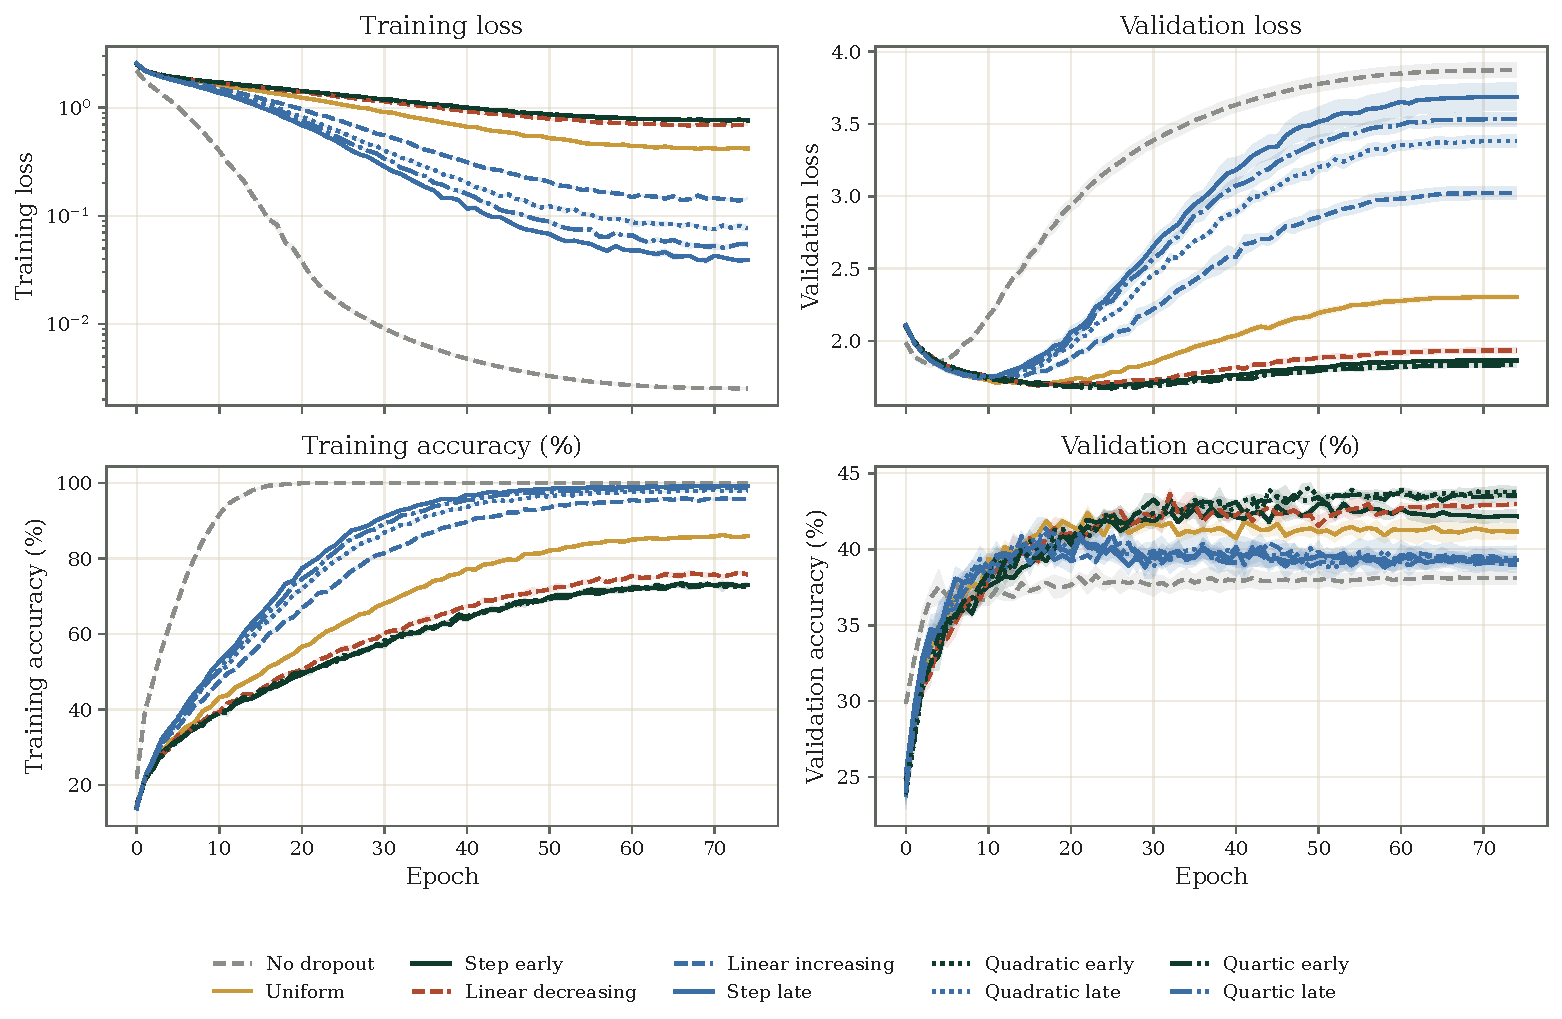
\includegraphics[width=0.94\textwidth]{figures/experiments/benchmarks/profile-geometry-pilot.pdf}
\caption{Profile geometry at fixed mean dropout. Training and validation curves use the original paper style and show mean $\pm$ SEM over three seeds.}
\label{fig:profile-geometry-pilot}\end{figure}
\begin{center}\small\begin{tabular}{@{}lrr@{}}\toprule
Profile & Final validation CE & Final validation accuracy (\%) \\
\midrule
No dropout & \(3.872\pm0.053\) & \(38.10\pm0.40\) \\
Uniform & \(2.303\pm0.019\) & \(41.17\pm0.55\) \\
Step early & \(1.864\pm0.009\) & \(42.17\pm0.43\) \\
Linear decreasing & \(1.933\pm0.019\) & \(42.97\pm0.15\) \\
Linear increasing & \(3.025\pm0.045\) & \(39.30\pm0.40\) \\
Step late & \(3.688\pm0.097\) & \(39.27\pm0.30\) \\
Quadratic early & \(1.852\pm0.001\) & \(43.73\pm0.38\) \\
Quadratic late & \(3.382\pm0.042\) & \(39.43\pm0.80\) \\
Quartic early & \(1.831\pm0.016\) & \(43.53\pm0.41\) \\
Quartic late & \(3.534\pm0.048\) & \(39.00\pm0.50\) \\
\bottomrule\end{tabular}\end{center}
The saved records do not contain a complete width-transfer comparison. The geometry pilot alone does not establish successful $\mu$P transfer.
